% !TEX root = ../OT4ML.tex


%%%%%%%%%%%%%%%%%%%%%%%%%%%%%%%%%%%%%%%%%%%%%%%%%%%%%%%%%%%%%%%%%%%%%%%%%%%
%%%%%%%%%%%%%%%%%%%%%%%%%%%%%%%%%%%%%%%%%%%%%%%%%%%%%%%%%%%%%%%%%%%%%%%%%%%
%%%%%%%%%%%%%%%%%%%%%%%%%%%%%%%%%%%%%%%%%%%%%%%%%%%%%%%%%%%%%%%%%%%%%%%%%%%
\chapter{Entropic Regularization: Sinkhorn Algorithm}
\index{entropic!regularization}% strictindex
\index{Sinkhorn!algorithm}% strictindex
\label{sec-sinkhorn}

Entropic regularization makes optimal transport smooth, strictly convex and scalable. This chapter first explains the discrete KL-regularized problem, derives Sinkhorn's alternating matrix scaling algorithm, and then rewrites the same construction as a relative-entropy projection problem. It then records the general continuous formulation, develops the dual soft-transform picture, and presents the main convex regularization variants and the debiased Sinkhorn divergence. Its stochastic path-space interpretation is developed later, alongside dynamic OT, in Section~\ref{sec-path-space-schrodinger}. A final section records a less standard viewpoint: after fixing the potential gauge, the finite-dimensional Sinkhorn equations admit a local holomorphic continuation to complex values of the temperature. The presentation connects the older matrix-scaling literature~\cite{Sinkhorn64,SinkhornKnopp67,Sinkhorn67} with modern entropic OT~\cite{CuturiSinkhorn,peyre2019computational}.
\index{matrix!scaling}% strictindex
\index{entropic!OT}% strictindex
\index{path-space formulation}% strictindex
\index{Schrodinger@Schr\"odinger!problem}% strictindex
\index{entropic!regularization}% strictindex
\index{Sinkhorn!divergence}% strictindex
\index{scaling!algorithm}% strictindex
\index{relative!entropy}% strictindex
\index{soft!transform}% strictindex
\index{Sinkhorn!scaling}% strictindex

%%%%%%%%%%%%%%%%%%%%%%%%%%%%%%%%%%%%%%%%%%%%%%%%%%%%%%%%%%%%%%%%%%%%%%%%%%%
\section{Entropic Regularization for Discrete Measures}
\index{entropic!regularization}% strictindex
\index{discrete!measure}% strictindex
\label{sec-entropic-discrete}

Entropy turns a possibly non-unique linear program into a unique smooth problem. The price is bias, but the reward is differentiability and fast scaling algorithms.
\index{scaling!algorithm}% strictindex

\paragraph{Entropy penalty.}
\index{entropy!penalty}% strictindex
The idea of the entropic regularization of optimal transport is to penalize concentrated couplings by adding the negative of the discrete Shannon--Boltzmann entropy.
\index{Shannon-Boltzmann entropy}% strictindex

\begin{defn}[Discrete Shannon--Boltzmann entropy]\label{def-discrete-shannon-boltzmann-entropy}
\index{Shannon entropy}% strictindex
\index{Boltzmann entropy}% strictindex
	For a nonnegative matrix $\P$, its Shannon--Boltzmann entropy is
	\[
		\HD(\P) \eqdef -\sum_{i,j} \P_{i,j} \log(\P_{i,j}),
	\]
	with the convention $0\log(0)=0$.
\end{defn}
Using this entropy as a regularizing function gives approximate solutions to the original transport problem~\eqref{eq-kanto-discr}
\eql{\label{eq-regularized-discr}
	\MKD_\C^\epsilon(\a,\b) \eqdef
	\umin{\P \in \CouplingsD(\a,\b)}
		\dotp{\P}{\C} - \epsilon \HD(\P).
}

\begin{prop}[Existence and uniqueness of entropic OT]\label{prop-entropic-unique}
\index{entropic!OT}% strictindex
	Assume that $\a,\b$ are probability histograms and that $\C$ is finite. For every $\epsilon>0$, problem~\eqref{eq-regularized-discr} admits a unique minimizer. If all entries of $\a$ and $\b$ are positive, then this minimizer is positive on every entry.
\index{histogram}% strictindex
\end{prop}

\begin{proof}
	The transport polytope $\CouplingsD(\a,\b)$ is non-empty and compact, and the objective is continuous on it with the convention $0\log0=0$, so a minimizer exists. The scalar function $r\mapsto r\log r$ is strictly convex on $[0,+\infty)$. On the relative interior, the Hessian
\index{transportation polytope}% strictindex
	\[
		-\partial^2 \HD(\P)=\diag(1/\P_{i,j})
	\]
	is positive definite. Hence $-\HD$ is strictly convex on every nontrivial feasible segment, and $\dotp{\P}{\C}-\epsilon\HD(\P)$ has at most one minimizer.

	If $\a_i,\b_j>0$ and a minimizer had $\P_{i,j}=0$, then for small $t>0$ the perturbation $\P_t=(1-t)\P+t\,\a\otimes\b$ remains feasible. The directional derivative of the entropic part at $t=0$ is $-\infty$ because the derivative of $r\log r$ at $0$ is $-\infty$ along a positive direction. Thus the objective decreases for small $t$, contradicting optimality. Therefore the minimizer is strictly positive.
\end{proof}


%%%%%
\paragraph{Smoothing effect.}
\index{entropic!smoothing}% strictindex

By Proposition~\ref{prop-entropic-unique}, problem~\eqref{eq-regularized-discr} has a unique optimal solution.
%
Beyond providing uniqueness, this smoothing makes $\MKD_\C^\epsilon(\a,\b)$ a smooth function of $\a$, $\b$ and $\C$ whenever these variables remain in the relative interior of their domains. In finite dimension, this follows from the smooth dual problem, which is strictly concave after fixing its additive gauge, and the envelope theorem.
\index{envelope theorem}% strictindex
\index{strict!convexity}% strictindex
\index{dual!problem}% strictindex
%
The entropy acts as a barrier for the positivity constraint: Proposition~\ref{prop-entropic-unique} shows that the solution is strictly positive on the support of $\a\otimes\b$. At the opposite, high-temperature end, Proposition~\ref{prop-convergence-eps} shows that $\P_\epsilon\to\a\otimes\b$ as $\epsilon\to+\infty$.

Figure~\ref{fig:sinkhorn-entropy-lp-geometry} visualizes this entropic path on a transport-polytope slice and compares it with entropy applied to the slack variables of a generic linear program.

\begin{figure}[H]
\centering
\setlength{\tabcolsep}{2pt}
\begin{tabular}{@{}cccc@{}}
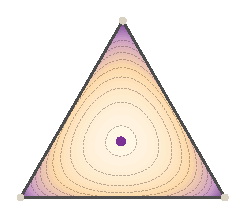
\includegraphics[width=.21\linewidth]{figures/sinkhorn-entropy-lp-geometry--eps-large.pdf} &
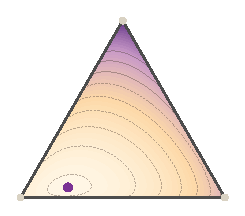
\includegraphics[width=.21\linewidth]{figures/sinkhorn-entropy-lp-geometry--eps-medium.pdf} &
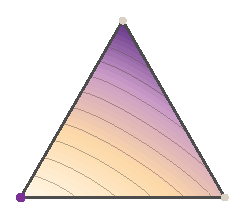
\includegraphics[width=.21\linewidth]{figures/sinkhorn-entropy-lp-geometry--eps-small.pdf} &
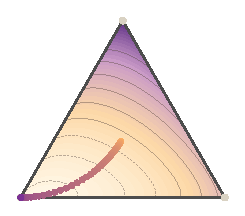
\includegraphics[width=.21\linewidth]{figures/sinkhorn-entropy-lp-geometry--path.pdf} \\[-.1em]
\small large $\epsilon$ &
\small medium $\epsilon$ &
\small small $\epsilon$ &
\small entropic path \\[.35em]
\index{entropic!path}% strictindex
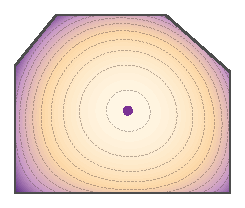
\includegraphics[width=.21\linewidth]{figures/sinkhorn-entropy-lp-geometry--barrier-large.pdf} &
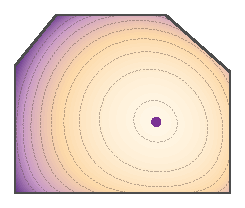
\includegraphics[width=.21\linewidth]{figures/sinkhorn-entropy-lp-geometry--barrier-medium.pdf} &
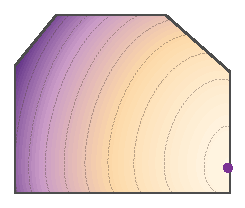
\includegraphics[width=.21\linewidth]{figures/sinkhorn-entropy-lp-geometry--barrier-small.pdf} &
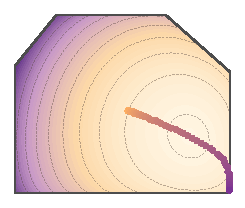
\includegraphics[width=.21\linewidth]{figures/sinkhorn-entropy-lp-geometry--barrier-path.pdf} \\[-.1em]
\small LP slack barrier &
\small intermediate &
\small low temperature &
\small barrier path
\end{tabular}
\caption{\emph{Entropic regularization and slack barriers.} The first row shows the penalized objective $\dotp{c}{p}+\epsilon\sum_i p_i(\log p_i-1)$ on a triangular face of the transport polytope; color and level sets represent the regularized functional itself, not only the linear part. The second row shows the analogous entropy-on-slacks objective $\ell^\top z+\epsilon H(b-Az)$ on a two-dimensional polyhedron $Az\leq b$, with $H(s)=\sum_i s_i(\log s_i-1)$. Large $\epsilon$ selects an interior reference point, while small $\epsilon$ moves the minimizer toward a low-cost face.}
\index{entropic!regularization}% strictindex
\index{transportation polytope}% strictindex
\label{fig:sinkhorn-entropy-lp-geometry}
\end{figure}

\begin{rem}[Entropy barriers versus generic LP barriers]\label{rem-entropy-versus-lp-barriers}
\index{barrier!entropy}% strictindex
\index{barrier!LP}% strictindex
For a generic linear program $\min_z \ell^\top z$ subject to $Az\leq b$, one can introduce positive slacks $s=b-Az$ and use an entropy-on-slacks penalty $H(s)=\sum_i s_i(\log s_i-1)$ as a smooth interior regularization. This is a useful analogy for Figure~\ref{fig:sinkhorn-entropy-lp-geometry}, but it is not the standard interior-point barrier for linear programming. The canonical barrier on the positive orthant is the Burg, or reverse-KL, logarithmic barrier $-\sum_i\log s_i$; it is self-concordant and therefore fits the Newton theory of interior-point methods~\cite{nesterov1994interior}. The price is that a generic Newton step solves a dense linear system, leading to cubic per-iteration scaling in the relevant number of variables or constraints. Optimal transport is special: the entropy is placed on the entries of $\P$, while the constraints are only the row and column marginals. This separable structure turns the associated Bregman projections into diagonal rescalings, hence into the Sinkhorn matrix-vector iterations developed next.
\index{Newton step}% strictindex
\index{self-concordance}% strictindex
\index{dense linear system}% strictindex
\index{matrix-vector iteration}% strictindex
\index{linear!programming}% strictindex
\index{interior-point method}% strictindex
\index{barrier!logarithmic}% strictindex
\index{Bregman!projection}% strictindex
\index{Sinkhorn!algorithm}% strictindex
\end{rem}


%%%%%%%%%%%%%%%%%%%%%%%%%%%%%%%%%%%%%%%%%%%%%%%%%%%%%%%%%%%%%%%%%%%%%%%%%%%

%%%%%%%%%%%%%%%%%%%%%%%%%%%%%%%%%%%%%%%%%%%%%%%%%%%%%%%%%%%%%%%%%%%%%%%%%%%
\section{Sinkhorn's Algorithm}


Sinkhorn's algorithm is alternating normalization of rows and columns. This section derives the scaling form of the optimizer and explains why each iteration only needs matrix-vector products.
\index{scaling!form}% strictindex
\index{Sinkhorn!scaling}% strictindex

The underlying matrix-scaling iteration has a long history, including iterative proportional fitting and the work of Sinkhorn and Knopp~\cite{Sinkhorn64,SinkhornKnopp67,Sinkhorn67}. Its modern role in OT was transformed by Cuturi's entropic formulation~\cite{CuturiSinkhorn}: the algorithm became a practical large-scale tool for machine learning, and also changed the way OT is viewed in ML, from a mostly geometric distance to a differentiable computational primitive.
\index{iterative proportional fitting}% strictindex
\index{matrix!scaling}% strictindex

The following proposition shows that the solution of~\eqref{eq-regularized-discr} has a specific form. The parameterization is essentially dual: a coupling has $nm$ entries and $n+m-1$ independent marginal constraints, whereas the two scaling vectors use $n+m$ variables modulo one multiplicative gauge.

\begin{prop}[Scaling form of entropic OT]\label{prop-regularized-primal}
\index{scaling!form}% strictindex
\index{entropic!OT}% strictindex
$\P$ is the unique solution to~\eqref{eq-regularized-discr} if and only if there exists $(\uD,\vD) \in \RR_+^n \times \RR_+^m$ such that
\eql{\label{eq-scaling-form}
	\foralls (i,j) \in \range{n} \times \range{m}, \quad \P_{i,j} = \uD_i \K_{i,j} \vD_j
		\qwhereq \K_{i,j} \eqdef e^{-\frac{\C_{i,j}}{\epsilon}},
}
and $\P \in \CouplingsD(\a,\b)$.
\end{prop}

\begin{proof}
	Without loss of generality, we assume $\a_i,\b_j>0$ (otherwise, rows or columns with zero mass are fixed to zero and can be removed). By Proposition~\ref{prop-entropic-unique}, the minimizer is strictly positive on the remaining support.
\index{zero mass}% strictindex

	We can thus ignore the positivity constraint when introducing two dual variables $\fD\in\RR^n,\gD\in\RR^m$ for each marginal constraint so that the Lagrangian of~\eqref{eq-regularized-discr} reads
\index{marginal!constraint}% strictindex
	\eq{\label{eq-sinkhorn-lagrangian}
		\Lag(\P,\fD,\gD)=
		\dotp{\P}{\C}
		+\epsilon\sum_{i,j}\P_{i,j}\log(\P_{i,j})
		+ \dotp{\fD}{\a - \P\ones_m}
		+ \dotp{\gD}{\b - \transp{\P}\ones_n}.
	}
	The first-order conditions are

\[
		\frac{\partial\Lag(\P,\fD,\gD)}{\partial \P_{i,j}}= \C_{i,j} + \epsilon (\log\pa{ \P_{i,j} }+1) - \fD_i -\gD_j = 0.
\]
Thus
$\P_{i,j}=e^{(\fD_i+\gD_j-\C_{i,j})/\epsilon-1}$,
which has the stated form with the positive scalings
$\uD_i\eqdef e^{\fD_i/\epsilon-1}$ and $\vD_j\eqdef e^{\gD_j/\epsilon}$.
\end{proof}

The factorization in~\eqref{eq-scaling-form} can be written compactly as $\P=\diag(\uD)\K\diag(\vD)$.
\index{scaling!form}% strictindex
%
$\uD,\vD$ must therefore satisfy the nonlinear mass-conservation equations
\index{mass!conservation}% strictindex
\eql{\label{eq-dualsinkhorn-constraints}
	\diag(\uD)\K\diag(\vD)\ones_m=\a,
	\qandq
	\diag(\vD)\K^\top \diag(\uD)\ones_n=\b,
}
Using entrywise multiplication, these equations reduce to
\eql{\label{eq-dualsinkhorn-constraints2}
	\uD \odot (\K \vD) = \a
	\qandq
	\vD \odot (\transp{\K}\uD) = \b
}
where $\odot$ denotes entrywise multiplication. This is the matrix-scaling problem; see~\cite{nemirovski1999complexity} and the references therein.
\index{matrix!scaling}% strictindex

Diagonal normalization of a positive matrix has a long history, from iterative proportional fitting in statistics and economics~\cite{kruithof,yule1912methods,Galichon-Entropic} to modern matrix-balancing algorithms~\cite{ReviewSinkhorn,cohen2017matrix}.
\index{iterative proportional fitting}% strictindex
%
When $n=m$ and $\a,\b$ are uniform, this is diagonal scaling toward bistochasticity. Proposition~\ref{prop-entropic-unique} guarantees a unique scaled matrix $\P$, although the two scaling vectors retain one multiplicative gauge degree of freedom. If some entries of $\K$ vanish, equivalently if $\C$ can take the value $+\infty$, existence and uniqueness require additional support conditions; here we keep $\K>0$.
\index{cost!matrix}% strictindex


Sinkhorn's algorithm solves the two equations alternately: it first updates $\uD$ to enforce the source marginal and then updates $\vD$ to enforce the target marginal,
\index{Sinkhorn!algorithm}% strictindex
\eql{\label{eq-sinkhorn}
	\itt{\uD} \eqdef \frac{\a}{\K \it{\vD}}
	\qandq
	\itt{\vD} \eqdef \frac{\b}{\transp{\K}\itt{\uD}},
}
initialized with any positive vector, for instance $\init{\vD}=\ones_m$. Division is entrywise. Different initializations may select different representatives of the same scaling class, because $(\lambda\uD,\vD/\lambda)$ yields the same coupling for every $\lambda>0$.
%
The alternating normalization can be read directly on the coupling matrix: a row update enforces the source marginal and generally perturbs the target marginal, while the next column update does the converse.

\begin{alg}[Sinkhorn scaling]\label{alg:sinkhorn-scaling}
\textbf{Input:} Positive weights $\a,\b$, cost matrix $\C$, regularization $\epsilon>0$, tolerance $\mathrm{tol}$.

\textbf{Output:} Entropic coupling $\P$.

\textbf{Initialize:} Set $\K_{ij}=e^{-\C_{ij}/\epsilon}$, $\vD^{(0)}=\ones_m$, \(r^{(0)}=+\infty\), and \(\ell=0\).

\textbf{While} \(r^{(\ell)}>\mathrm{tol}\) \textbf{do}:
\begin{algblock}

\textbf{Set} \(\ell\leftarrow \ell+1\).

\(\uD^{(\ell)}=\frac{\a}{\K\vD^{(\ell-1)}}.\)

\(\vD^{(\ell)}=\frac{\b}{\transp{\K}\uD^{(\ell)}}.\)

\(\P^{(\ell)}=\diag(\uD^{(\ell)})\K\diag(\vD^{(\ell)}).\)

\textbf{Set} \(r^{(\ell)}=\max\{\norm{\P^{(\ell)}\ones_m-\a}_1,\norm{(\P^{(\ell)})^\top\ones_n-\b}_1\}\).
\end{algblock}
\algreturnskip
\textbf{Return} \(\P^{(\ell)}\).
\end{alg}

Figure~\ref{fig:sinkhorn-marginal-errors} exposes the alternating feasibility mechanism on a small matrix: each row or column normalization enforces one marginal exactly while generally perturbing the other.

\begin{figure}[H]
\centering
\setlength{\tabcolsep}{1.5pt}
\begin{tabular}{@{}ccccc@{}}
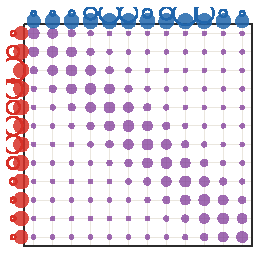
\includegraphics[width=.18\linewidth]{figures/sinkhorn-marginal-errors--initial.pdf} &
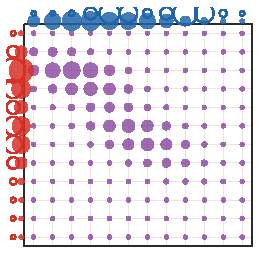
\includegraphics[width=.18\linewidth]{figures/sinkhorn-marginal-errors--row-1.pdf} &
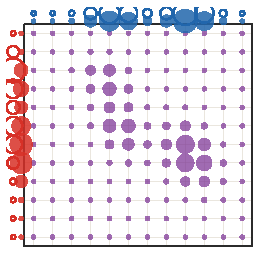
\includegraphics[width=.18\linewidth]{figures/sinkhorn-marginal-errors--column-1.pdf} &
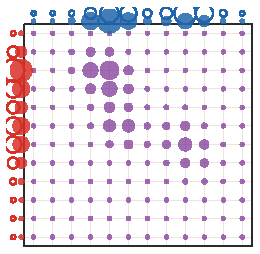
\includegraphics[width=.18\linewidth]{figures/sinkhorn-marginal-errors--row-2.pdf} &
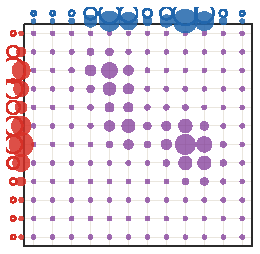
\includegraphics[width=.18\linewidth]{figures/sinkhorn-marginal-errors--column-2.pdf} \\[-.1em]
\small initial $K$ &
\small row 1 &
\small column 1 &
\small row 2 &
\small column 2
\end{tabular}
\caption{\emph{Marginal constraints during Sinkhorn scaling on a twelve-bin one-dimensional problem.} Violet circles represent the current coupling matrix, framed by the thin black box; the red source marginal is displayed on the left and the blue target marginal below the matrix. Hollow side circles show the prescribed marginals, while filled circles show the current marginals. Row normalizations align the red marginal and leave a blue defect; column normalizations align the blue marginal and leave a red defect.}
\index{row normalization}% strictindex
\index{column normalization}% strictindex
\index{Sinkhorn!scaling}% strictindex
\index{marginal!constraint}% strictindex
\label{fig:sinkhorn-marginal-errors}
\end{figure}

The same alternating projection mechanism is clearer on a dense one-dimensional discretization, where the marginal defects appear as continuous side curves.
\index{alternating!projection}% strictindex

Figure~\ref{fig:sinkhorn-continuous-marginal-scaling} shows the same alternating projection mechanism on a dense one-dimensional discretization, where the marginal defects appear as continuous side curves.

\begin{figure}[H]
\centering
\begin{tabular}{@{}cccc@{}}
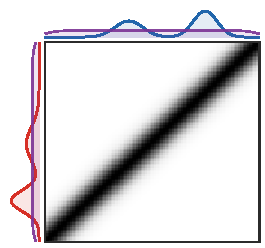
\includegraphics[width=.22\linewidth]{figures/sinkhorn-continuous-marginal-scaling--initial.pdf} &
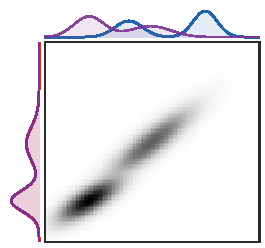
\includegraphics[width=.22\linewidth]{figures/sinkhorn-continuous-marginal-scaling--row-1.pdf} &
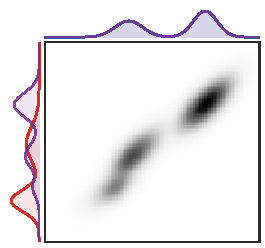
\includegraphics[width=.22\linewidth]{figures/sinkhorn-continuous-marginal-scaling--column-1.pdf} &
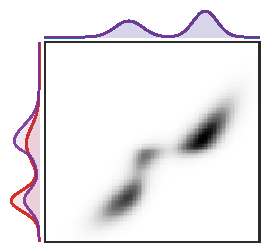
\includegraphics[width=.22\linewidth]{figures/sinkhorn-continuous-marginal-scaling--column-12.pdf} \\[-.1em]
\small initial $K$ &
\small after one row scaling &
\index{scaling!row}% strictindex
\small after one column scaling &
\index{scaling!column}% strictindex
\small after 12 cycles
\end{tabular}
\caption{\emph{Dense Sinkhorn scaling for one-dimensional Gaussian-mixture marginals.} The grayscale matrix is the current coupling, with a thin box delimiting only the matrix and not the side marginal plots. The red and blue side curves are the prescribed source and target marginals, while the violet side curves are the current row and column sums. A row scaling makes the violet curve coincide with the red source marginal, a column scaling makes it coincide with the blue target marginal, and the alternation rapidly stabilizes both sides.}
\index{Sinkhorn!scaling}% strictindex
\index{Gaussian!mixture}% strictindex
\label{fig:sinkhorn-continuous-marginal-scaling}
\end{figure}

After convergence, the regularization strength controls how much of the Gibbs kernel remains visible in the optimal plan. Small $\epsilon$ produces a concentrated transport band, while larger $\epsilon$ spreads the same marginals into a smoother coupling.
\index{optimal plan}% strictindex
\index{Gibbs!kernel}% strictindex

Figure~\ref{fig:sinkhorn-coupling-iterations} compares these converged plans at four temperatures while keeping both marginals fixed.

\begin{figure}[H]
\centering
\begin{tabular}{@{}cccc@{}}
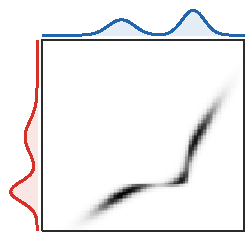
\includegraphics[width=.215\linewidth]{figures/sinkhorn-coupling-iterations--eps-0p010.pdf} &
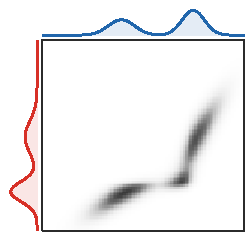
\includegraphics[width=.215\linewidth]{figures/sinkhorn-coupling-iterations--eps-0p030.pdf} &
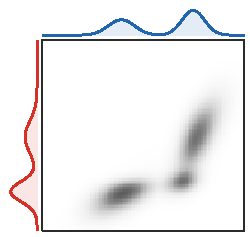
\includegraphics[width=.215\linewidth]{figures/sinkhorn-coupling-iterations--eps-0p085.pdf} &
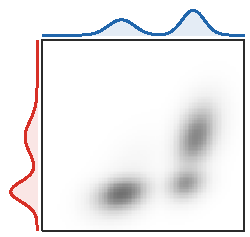
\includegraphics[width=.215\linewidth]{figures/sinkhorn-coupling-iterations--eps-0p240.pdf} \\[-.1em]
\small $\epsilon=0.010$ &
\small $\epsilon=0.030$ &
\small $\epsilon=0.085$ &
\small $\epsilon=0.240$
\end{tabular}
\caption{\emph{Final Sinkhorn couplings for the same one-dimensional Gaussian-mixture marginals and four regularization strengths.} Each boxed matrix is the converged solution of the KL-regularized problem and uses a common grayscale normalization; the side curves display the fixed source and target marginals. Decreasing $\epsilon$ sharpens the plan toward an optimal-transport graph, whereas increasing $\epsilon$ keeps more of the diffuse product-measure structure.}
\index{Gaussian!mixture}% strictindex
\index{product!measure}% strictindex
\label{fig:sinkhorn-coupling-iterations}
\end{figure}

Chapter~\ref{sec-entropic-convergence} gives the formal convergence analysis. Before that, Figure~\ref{fig:sinkhorn-potentials-iterations} tracks the same Sinkhorn scaling in dual variables. The logarithmic row and column scalings, normalized to fix their additive gauge, rapidly settle to stable Kantorovich--Sinkhorn potentials.
\index{dual!potential}% strictindex

\begin{figure}[ht]
\centering
\setlength{\tabcolsep}{2pt}
\begin{tabular}{@{}cccc@{}}
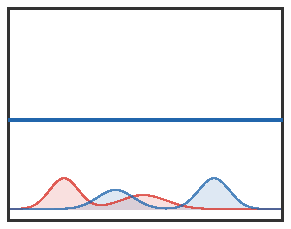
\includegraphics[width=.23\linewidth]{figures/sinkhorn-potentials-iterations--iter-0.pdf} &
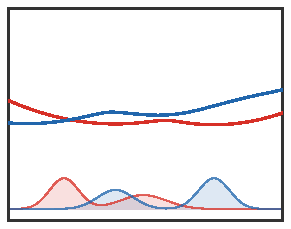
\includegraphics[width=.23\linewidth]{figures/sinkhorn-potentials-iterations--iter-1.pdf} &
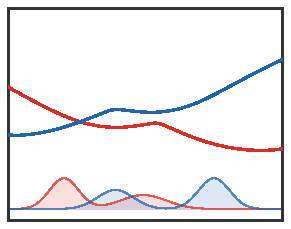
\includegraphics[width=.23\linewidth]{figures/sinkhorn-potentials-iterations--iter-3.pdf} &
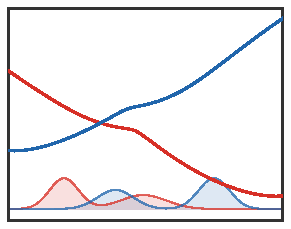
\includegraphics[width=.23\linewidth]{figures/sinkhorn-potentials-iterations--iter-12.pdf} \\[-.1em]
\small $k=0$ &
\small $k=1$ &
\small $k=3$ &
\small $k=12$
\end{tabular}
\caption{\emph{KL-normalized Sinkhorn dual potentials along Sinkhorn scaling.} The setting is the same one-dimensional Gaussian-mixture problem as Figure~\ref{fig:sinkhorn-dual-potentials-epsilon}, with fixed regularization strength $\epsilon=0.045$. The bottom silhouettes show both the source histogram $\a$ in red and the target histogram $\b$ in blue, while the red and blue curves are the logarithmic scaling potentials. All panels share the same axes, making stabilization visible.}
\index{scaling!potential}% strictindex
\index{Gaussian!mixture}% strictindex
\index{dual!potential}% strictindex
\label{fig:sinkhorn-potentials-iterations}
\end{figure}

Complexity bounds for Sinkhorn and comparisons with accelerated first-order methods are discussed in~\cite{altschuler2017near,pmlr-v80-dvurechensky18a,knight2008sinkhorn}.
%
A chief computational advantage of Sinkhorn's algorithm, besides its simplicity, is that the only expensive operation is multiplication by the Gibbs kernel. With a dense $n\times m$ kernel, $N_{\rm it}$ iterations therefore cost $O(N_{\rm it}nm)$. Chapter~\ref{sec-convergence-dual} gives a more precise convergence statement: for fixed $\epsilon$, the entropic dual gap has an $O(1/\ell)$ bound with a constant proportional to $1/\epsilon$, while Hilbert-metric arguments give linear convergence when the Gibbs kernel is uniformly positive. Approximating unregularized OT also requires balancing optimization error against entropic bias. In finite dimension, choosing $\epsilon$ of order $\delta$ and solving the regularized problem to accuracy of order $\delta$ leads to an iteration bound of order $1/\delta^2$, up to logarithmic and cost-range factors~\cite{altschuler2017near,pmlr-v80-dvurechensky18a}.
\index{dual!gap}% strictindex
\index{Sinkhorn!iteration}% strictindex
\index{Sinkhorn!algorithm}% strictindex
\index{linear!convergence}% strictindex
\index{entropic!bias}% strictindex
\index{Gibbs!kernel}% strictindex

Figure~\ref{fig:sinkhorn-linear-rate-epsilon} complements the complexity discussion by plotting the marginal defect across half-steps and showing how smaller temperatures slow the observed linear regime.

\begin{figure}[H]
\centering
\setlength{\tabcolsep}{3pt}
\begin{tabular}{@{}cc@{}}
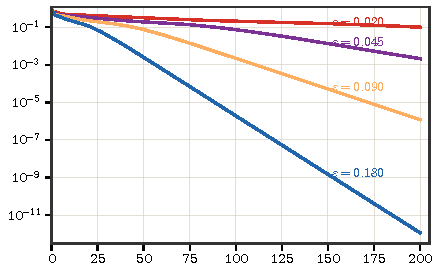
\includegraphics[width=.58\linewidth]{figures/sinkhorn-linear-rate-epsilon--marginal-error.pdf} &
\raisebox{.75em}{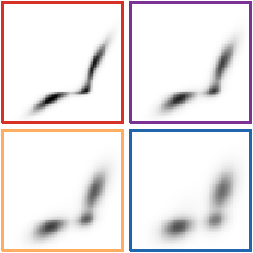
\includegraphics[width=.31\linewidth]{figures/sinkhorn-linear-rate-epsilon--limiting-plans.pdf}} \\[-.1em]
\small marginal violation &
\small limiting plans $\P_\epsilon$
\end{tabular}
\caption{\emph{Marginal violation along Sinkhorn half-steps.} The four curves use the same one-dimensional Gaussian-mixture problem and are paired with the corresponding limiting plans. The plotted error is $\frac12(\|\P^{(\ell)}\ones-\a\|_1+\|(\P^{(\ell)})^\top\ones-\b\|_1)$ on a logarithmic scale. The colored boxes on the right use the same colors as the convergence curves. For fixed positive $\epsilon$, the curves enter a linear regime; smaller $\epsilon$ gives a sharper transport geometry but a more peaked Gibbs kernel and slower scaling.}
\index{Sinkhorn!half-step}% strictindex
\index{Gaussian!mixture}% strictindex
\index{Gibbs!kernel}% strictindex
\label{fig:sinkhorn-linear-rate-epsilon}
\end{figure}

In many applications, however, one does not need a highly accurate optimizer for the OT subproblem. Downstream performance is often tied more to the geometric bias of the discrepancy than to exact optimality, so a moderate number of iterations can suffice.
%
This should be contrasted with generic interior-point methods, which use logarithmic barriers and require solving Newton systems. A dense transportation problem has $nm$ primal variables, so a naive dense factorization can cost $O((nm)^3)$ per Newton step, or $O(n^6)$ when $n=m$. The overall complexity also depends on the formulation, sparsity, conditioning and iteration bound; the per-step comparison, rather than a universal total bound, is the relevant point here.
\index{interior-point method}% strictindex
\index{barrier!logarithmic}% strictindex

The second crucial aspect of Sinkhorn is that matrix-vector multiplication streams extremely well on GPU. Even better, if one is interested in computing many OT problems with a fixed cost matrix $\C$, one can replace many matrix-vector multiplications with matrix-matrix multiplications, so that the computational gain can be substantial.
\index{cost!matrix}% strictindex

\begin{rem}[Separable Gaussian kernels on grids]\label{rem-sinkhorn-separable-gaussian}
\index{kernel!Gaussian}% strictindex
	When the samples lie on a Cartesian grid and $c(x,y)=\norm{x-y}^2$, the Gibbs kernel is Gaussian and factorizes along coordinates. If the grid has $q$ points per axis in dimension $d$, so that $N=q^d$ grid points are used, then
\index{Gibbs!kernel}% strictindex
	\[
		K(x,y)=\exp\!\left(-\frac{\norm{x-y}^2}{\epsilon}\right)
		=
		\prod_{\ell=1}^d
		\exp\!\left(-\frac{(x_\ell-y_\ell)^2}{\epsilon}\right).
	\]
	Multiplication by $K$ can therefore be applied by successively multiplying along each coordinate direction, equivalently by applying one-dimensional Gaussian kernel operators along the axes. On a periodic or sufficiently padded uniform grid these are literal discrete convolutions. A direct dense one-dimensional multiplication costs $O(q^2)$ on each of the $q^{d-1}$ coordinate lines, and this is repeated for $d$ axes. Hence one Sinkhorn half-step costs
\index{Sinkhorn!half-step}% strictindex
\index{kernel!Gaussian}% strictindex
	\begin{equation}\label{eq-separable-gaussian-half-step}
		O(d\,q^{d+1})=O(d\,N^{1+1/d})
	\end{equation}
	instead of $O(N^2)$. With FFT-based or truncated Gaussian convolutions, the same separability can be pushed further, but the simple tensor-product estimate already explains why grid-based Sinkhorn can scale much better than a generic dense coupling.
\end{rem}



%%%%%%%%%%%%%%%%%%%%%%%%%%%%%%%%%%%%%%%%%%%%%%%%%%%%%%%%%%%%%%%%%%%%%%%%%%%
\section{Reformulation Using Relative Entropy}
\index{relative!entropy}% strictindex

The KL formulation identifies Sinkhorn as a projection method. It also prepares the continuous and unbalanced settings, where a reference measure is essential.
\index{reference!measure}% strictindex

A convenient tool to reformulate and ``normalize'' this discrete entropy is relative entropy. It is the finite-dimensional divergence that turns entropy regularization into a projection problem and admits a direct measure-theoretic extension.

\begin{defn}[Discrete relative entropy]\label{def-discrete-relative-entropy}
\index{Kullback-Leibler divergence}% strictindex
\index{relative!entropy}% strictindex
	For nonnegative matrices $\P,\Q$ of the same size, the generalized relative entropy, or Kullback--Leibler divergence, is
	\eql{\label{eq-kl-defn}
		\KLD(\P|\Q) \eqdef \sum_{i,j}  \P_{i,j} \log\pa{\frac{\P_{i,j}}{\Q_{i,j}}} - \P_{i,j} + \Q_{i,j}.
	}
	The convention is $0\log(0)=0$, and $\KLD(\P|\Q)=+\infty$ if there exists $(i,j)$ such that $\Q_{i,j}=0$ but $\P_{i,j} \neq 0$.
\end{defn}
For the specific case of comparing probability distributions, where $\P$ and $\Q$ have the same total mass, this further simplifies to
\eq{
	\KLD(\P|\Q) = \sum_{i,j}  \P_{i,j} \log\pa{\frac{\P_{i,j}}{\Q_{i,j}}}.
}
For the reference matrix $\Q=\ones_{n \times m}$, one has
\eq{
	-\KLD(\P|\ones_{n \times m})
	=
	\HD(\P)+\sum_{i,j}\P_{i,j}-n\,m .
}
On fixed-mass couplings the last two terms are constant, so KL regularization with reference $\ones_{n\times m}$ is equivalent to subtracting Shannon--Boltzmann entropy.
$\KLD$ is a particular instance of both a $\phi$-divergence (as defined in Section~\ref{sec-phi-div}) and a Bregman divergence; up to standard affine rescalings, it is the canonical overlap between these two families. This special property is at the heart of the fact that this regularization leads to elegant algorithms and a tractable mathematical analysis.
\index{Bregman!divergence}% strictindex
\index{phi-divergence}% strictindex

\begin{prop}[Non-negativity and definiteness of relative entropy]\label{prop-kl-distance-like}
\index{relative!entropy}% strictindex
	For all $\P,\Q\in\RR_+^{n\times m}$, one has $\KLD(\P|\Q)\geq0$, with equality if and only if $\P=\Q$.
\end{prop}
\begin{proof}
	Write $\phi(s)=s\log s-s+1$. Convexity gives $\phi(s)\geq \phi(1)+\phi'(1)(s-1)=0$, and strict convexity gives equality only at $s=1$. Hence
\index{strict!convexity}% strictindex
	\[
		\KLD(\P|\Q)=\sum_{(i,j):\,\Q_{i,j}>0}\Q_{i,j}
		\phi(\P_{i,j}/\Q_{i,j})\geq0,
	\]
	whenever $\P\ll\Q$ entrywise; otherwise the divergence is $+\infty$. Equality forces $\P_{i,j}=\Q_{i,j}$ wherever $\Q_{i,j}>0$, while entries with $\Q_{i,j}=0$ vanish in both matrices. Thus equality is equivalent to $\P=\Q$.
\end{proof}

When $\P$ and $\Q$ are probability matrices and $\P\ll\Q$, the same divergence can also be written
\eq{
	\KLD(\P|\Q)
	=\sum_{i,j}\psi(\P_{i,j}/\Q_{i,j})\Q_{i,j},
	\qquad \psi(s)=s\log s.
}
More generally, for any convex $\psi$ such that $\psi(1)=0$, Jensen's inequality gives
\index{Jensen inequality}% strictindex
\eq{
	\sum_{i,j}\psi(\P_{i,j}/\Q_{i,j})\Q_{i,j}
	\geq \psi\!\left(\sum_{i,j}\P_{i,j}\right)=\psi(1)=0.
}

For instance, one can use as reference measure the tensor product $\a \otimes \b = (\a_i \b_j)_{i,j}$ and consider
\index{reference!measure}% strictindex
\eql{\label{eq-regularized-discr-rescaled}
	\umin{\P \in \CouplingsD(\a,\b)}
		\dotp{\P}{\C} + \epsilon \KLD(\P|\a \otimes \b).
}
This normalization will matter again for unbalanced OT, where changing the reference measure is no longer merely a harmless notational choice.
\index{unbalanced!OT}% strictindex

For the balanced problem with fixed positive marginals, however, the choice of tensor-product reference does not affect the selected coupling: it only adds a constant to the objective, as shown in the following proposition. In particular,~\eqref{eq-regularized-discr-rescaled} and~\eqref{eq-regularized-discr} have the same unique solution.

\begin{prop}[Reference measure shift for KL]\label{prop-kl-shift}
\index{reference!measure}% strictindex
\index{Kullback-Leibler divergence}% strictindex
	After removing zero-mass rows and columns, assume that $\a,\a'\in\simplex_n$ and $\b,\b'\in\simplex_m$ have positive entries. For every $\P \in \CouplingsD(\a,\b)$, one has
\eq{
	\KLD(\P|\a \otimes \b) =
	\KLD(\P|\a' \otimes \b') - \KLD(\a|\a') - \KLD(\b|\b').
}
Consequently, for fixed positive marginals, changing the positive tensor-product reference measure only adds a constant on the transport polytope. In particular,~\eqref{eq-regularized-discr-rescaled} and~\eqref{eq-regularized-discr} have the same unique minimizer.
\index{transportation polytope}% strictindex
\index{reference!measure}% strictindex
\end{prop}

\begin{proof}
Expanding the logarithm and using the marginal constraints gives
\index{marginal!constraint}% strictindex
\begin{align*}
	\KLD(\P|\a\otimes\b)
	&=
	\KLD(\P|\a'\otimes\b')
	+
	\sum_i \a_i\log\frac{\a_i'}{\a_i}
	+
	\sum_j \b_j\log\frac{\b_j'}{\b_j} \\[.25em]
	&=
	\KLD(\P|\a'\otimes\b')
	-\KLD(\a|\a')-\KLD(\b|\b').
\end{align*}
\end{proof}

The tensor-product reference is nevertheless useful when supports vary, because it makes explicit which entries are allowed to vanish. It is also the normalization that passes cleanly to the continuous formulation below, where the reference measure is $\al\otimes\be$ rather than an ambient Lebesgue measure.
\index{Lebesgue measure}% strictindex
\index{reference!measure}% strictindex

Figure~\ref{fig:sinkhorn-dual-potentials-epsilon} shows how the corresponding KL-normalized dual potentials deform with temperature, from nearly hard Kantorovich potentials to smoother log-sum-exp profiles.

\begin{figure}[H]
\centering
\begin{tabular}{@{}ccc@{}}
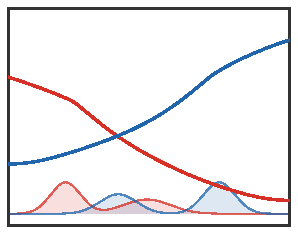
\includegraphics[width=.30\linewidth]{figures/sinkhorn-dual-potentials-epsilon--eps-0p010.pdf} &
\index{dual!potential}% strictindex
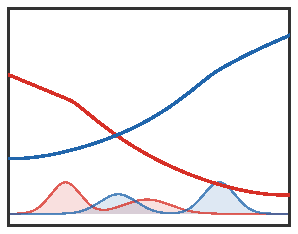
\includegraphics[width=.30\linewidth]{figures/sinkhorn-dual-potentials-epsilon--eps-0p045.pdf} &
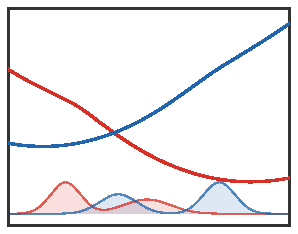
\includegraphics[width=.30\linewidth]{figures/sinkhorn-dual-potentials-epsilon--eps-0p200.pdf} \\[-.1em]
\small $\epsilon=0.010$ &
\small $\epsilon=0.045$ &
\small $\epsilon=0.20$
\end{tabular}
\caption{\emph{KL-normalized Sinkhorn dual potentials for the same one-dimensional Gaussian-mixture histograms.} The bottom silhouettes show both the source histogram $\a$ in red and the target histogram $\b$ in blue. The red and blue curves are the logarithmic scalings $\fD_i^\epsilon=\epsilon\log u_i^\epsilon$ and $\gD_j^\epsilon=\epsilon\log v_j^\epsilon$, with gauge $\dotp{\fD^\epsilon}{\a}=0$, computed from $\P_{i,j}=u_i\,\a_i\b_j e^{-\C_{i,j}/\epsilon}\,v_j$. The squared Euclidean cost is normalized by its median positive entry, and all panels use the same axes. For $\epsilon=0.010$ the curves are already close to the unregularized one-dimensional Kantorovich potentials; increasing $\epsilon$ turns this hard $c$-transform geometry into smoother log-sum-exp potentials.}
\index{Gaussian!mixture}% strictindex
\index{log-sum-exp}% strictindex
\index{dual!potential}% strictindex
\index{c-transform}% strictindex
\label{fig:sinkhorn-dual-potentials-epsilon}
\end{figure}


The KL-normalized formulation also makes the two limiting regimes of the regularization parameter transparent.

\begin{prop}[Convergence with $\epsilon$]\label{prop-convergence-eps}
	Assume, after removing zero-mass rows and columns, that $\a$ and $\b$ are positive and that $\C$ is finite.
	The unique solution $\P_\epsilon$ of~\eqref{eq-regularized-discr} converges to the optimal solution with maximal entropy within the set of all optimal solutions of the Kantorovich problem, namely
\index{Kantorovich!problem}% strictindex
\eql{\label{eq-entropy-conv-1}
	\P_\epsilon \overset{\epsilon \rightarrow 0}{\longrightarrow}
	\uargmin{\P} \enscond{ -\HD(\P) }{
		\P \in \CouplingsD(\a,\b), \dotp{\P}{\C} = \MKD_\C(\a,\b)
	}
}
so that in particular
\eq{
	\MKD_\C^\epsilon(\a,\b) \overset{\epsilon \rightarrow 0}{\longrightarrow} \MKD_\C(\a,\b).
}
Moreover,
\eql{\label{eq-entropy-conv-2}
	\P_\epsilon \overset{\epsilon \rightarrow \infty}{\longrightarrow}
	\a \otimes \b.
}
\end{prop}

\begin{proof}
	\textbf{Case $\epsilon \rightarrow 0$.}
	 We consider a sequence $(\epsilon_\ell)_\ell$ such that $\epsilon_\ell \rightarrow 0$ and $\epsilon_\ell > 0$.
	We denote $\P_\ell$ the solution of~\eqref{eq-regularized-discr} for $\epsilon=\epsilon_\ell$.
	%
	Since $\CouplingsD(\a,\b)$ is bounded, we can extract a sequence (that we do not relabel for the sake of simplicity) such that $\P_\ell \rightarrow \P^\star$. Since $\CouplingsD(\a,\b)$ is closed, $\P^\star \in \CouplingsD(\a,\b)$. We consider any $\P$ such that $\dotp{\C}{\P} = \MKD_\C(\a,\b)$. Using the equivalent KL-normalized formulation~\eqref{eq-regularized-discr-rescaled}, optimality of $\P$ and $\P_\ell$ for their respective optimization problems (for $\epsilon=0$ and $\epsilon=\epsilon_\ell$) gives
	\eql{\label{eq-proof-gamma-conv}
			0 \leq \dotp{\C}{\P_\ell} - \dotp{\C}{\P} \leq \epsilon_\ell ( \KLD(\P|\a \otimes \b)-\KLD(\P_\ell|\a \otimes \b) ).
		}
	Since $\KLD$ is continuous, taking the limit $\ell \rightarrow +\infty$ in this expression shows that
	$\dotp{\C}{\P^\star} = \dotp{\C}{\P}$ so that $\P^\star$ is a feasible point of~\eqref{eq-entropy-conv-1}. Furthermore, dividing by $\epsilon_\ell$ in~\eqref{eq-proof-gamma-conv} and taking the limit shows that
		$\KLD(\P^\star|\a \otimes \b) \leq \KLD(\P|\a \otimes \b)$, which shows that $\P^\star$ is a solution of~\eqref{eq-entropy-conv-1}. Since the solution $\P_0^\star$ to this program is unique by strict convexity of $\KLD(\cdot|\a \otimes \b)$ on the optimal face, one has $\P^\star = \P_0^\star$, and the whole sequence is converging.
\index{strict!convexity}% strictindex


\textbf{Case $\epsilon \rightarrow +\infty$.}
Subtracting $\min_{i,j}\C_{i,j}$ from the cost changes every feasible objective by the same constant, so it does not change the minimizer. We can therefore assume $\C\geq0$. Evaluating the energy at $\a \otimes \b$ (which belongs to the constraint set $\CouplingsD(\a,\b)$), one has
	\eq{
		\dotp{\C}{\P_\epsilon} + \epsilon \KLD(\P_\epsilon|\a \otimes \b) \leq \dotp{\C}{\a \otimes \b} + \epsilon \times 0
	}
	and since $\dotp{\C}{\P_\epsilon} \geq 0$, this leads to
	\eq{
		\KLD(\P_\epsilon|\a \otimes \b) \leq \epsilon^{-1} \dotp{\C}{\a \otimes \b} \leq \frac{\norm{\C}_\infty}{\epsilon}
	}
	so that $\KLD(\P_\epsilon|\a \otimes \b) \rightarrow 0$ and thus $\P_\epsilon \rightarrow \a \otimes \b$ since $\KLD$ is a valid divergence.
\end{proof}

Figure~\ref{fig:sinkhorn-plan-epsilon} illustrates the two limits of Proposition~\ref{prop-convergence-eps}: the plan approaches a sparse optimal coupling as $\epsilon\downarrow0$ and the product coupling as $\epsilon$ grows.

\begin{figure}[H]
\centering
\begin{tabular}{@{}cccc@{}}
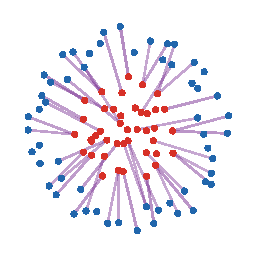
\includegraphics[width=.225\linewidth]{figures/sinkhorn-plan-epsilon--eps-0p018.pdf} &
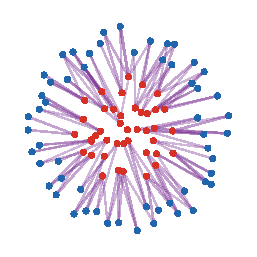
\includegraphics[width=.225\linewidth]{figures/sinkhorn-plan-epsilon--eps-0p045.pdf} &
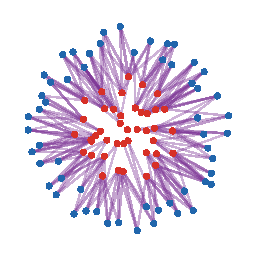
\includegraphics[width=.225\linewidth]{figures/sinkhorn-plan-epsilon--eps-0p120.pdf} &
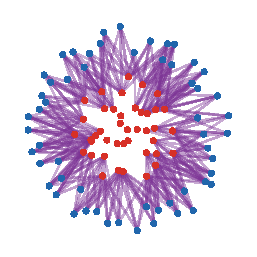
\includegraphics[width=.225\linewidth]{figures/sinkhorn-plan-epsilon--eps-0p320.pdf} \\[-.1em]
\small $\epsilon=0.018$ &
\small $\epsilon=0.045$ &
\small $\epsilon=0.120$ &
\small $\epsilon=0.320$
\end{tabular}
\caption{\emph{Entropically regularized couplings between the canonical red disk and blue annulus point clouds for four fixed regularization strengths.} The squared Euclidean cost is normalized by its median and each plan is computed by log-domain Sinkhorn until the marginal residual is below the notebook tolerance. Violet segments display the largest visible entries of the computed plan, with thickness and opacity proportional to transported mass. The plans are strictly positive for every $\epsilon>0$, but the visible mass pattern evolves from nearly radial and sparse to diffuse as $\epsilon$ increases.}
\index{log-domain Sinkhorn}% strictindex
\index{marginal!residual}% strictindex
\label{fig:sinkhorn-plan-epsilon}
\end{figure}

%%%%%%%%%%%%%%%%%%%%%%%%%%%%%%%%%%%%%%%%%%%%%%%%%%%%%%%%%%%%%%%%%%%%%%%%%%%

%%%%%%%%%%%%%%%%%%%%%%%%%%%%%%%%%%%%%%%%%%%%%%%%%%%%%%%%%%%%%%%%%%%%%%%%%%%
\section{General Formulation}

The continuous formulation replaces matrices by measures and discrete KL by relative entropy. This section records the measure-theoretic problem, explains how the temperature $\epsilon$ connects exact transport to the independent product coupling, and states the two asymptotic regimes that are useful later: a large-temperature expansion around independence and a small-temperature expansion around quadratic optimal transport.
\index{relative!entropy}% strictindex

\paragraph{Measure formulation.}

The only structural change from the discrete problem is that matrix entries are replaced by densities with respect to a reference product measure. This keeps the marginal constraints unchanged while turning the entropy into a relative entropy.

One can consider arbitrary measures by replacing the discrete entropy with the relative entropy with respect to the product measure $\d\al\otimes\d\be(x,y) \eqdef \d\al(x)\d\be(y)$, and propose a regularized counterpart to~\eqref{eq-mk-generic} using
\index{product!measure}% strictindex
\eql{\label{eq-entropic-generic}
	\MK_\c^\epsilon(\al,\be) \eqdef
	\umin{\pi \in \Couplings(\al,\be)}
		\int_{\X \times \Y} c(x,y) \d\pi(x,y) + \epsilon \KL(\pi|\al\otimes\be)
}
The measure-theoretic definition is the exact analogue of Definition~\ref{def-discrete-relative-entropy}, with absolute continuity replacing the entrywise support condition.

\begin{defn}[Relative entropy of measures]\label{def-measure-relative-entropy}
\index{Kullback-Leibler divergence}% strictindex
\index{relative!entropy}% strictindex
	For finite nonnegative measures $\pi$ and $\xi$ on $\Xx\times\Yy$, the relative entropy is
	\eql{\label{eq-defn-rel-entropy}
		\KL(\pi|\xi) \eqdef
		\int_{\Xx\times\Yy}\log\!\left(\frac{\d\pi}{\d\xi}\right)\d\pi
		+\xi(\Xx\times\Yy)-\pi(\Xx\times\Yy).
	}
		By convention, $\KL(\pi|\xi)=+\infty$ if $\pi$ is not absolutely continuous with respect to $\xi$.
\end{defn}
%
For fixed balanced marginals, the specific product reference in the entropy only matters up to additive constants, exactly as in Proposition~\ref{prop-kl-shift}. More precisely, an alternative product reference $\eta\otimes\zeta$ is admissible when $\al\ll\eta$, $\be\ll\zeta$ and the two marginal relative entropies are finite. The domination direction matters: a reference that fails to dominate a prescribed marginal gives infinite relative entropy. This distinction becomes substantive in the unbalanced setting, where the marginal constraints no longer freeze the additive terms.
\index{marginal!constraint}% strictindex
\index{absolute continuity}% strictindex

The dynamic counterpart of~\eqref{eq-entropic-generic} is the path-space Schr\"odinger problem developed in Section~\ref{sec-path-space-schrodinger}: it replaces an endpoint coupling by a probability law on noisy trajectories with the same prescribed endpoint marginals.

\paragraph{Probabilistic interpretation.}

The KL penalty has a simple statistical meaning: it measures how much dependence the coupling creates between its two marginals.

\begin{defn}[Mutual information]\label{def-mutual-information}
\index{mutual information}% strictindex
	If $(X,Y)\sim\pi$ have marginals $X\sim\al$ and $Y\sim\be$, the mutual information of the pair is
	\[
		\Ii(X,Y)\eqdef \KL(\pi|\al\otimes\be).
	\]
	It is nonnegative and vanishes if and only if $X$ and $Y$ are independent.
\end{defn}
With this terminology, the entropic problem~\eqref{eq-entropic-generic} is equivalent to
\[
	\inf_{X\sim\al,\;Y\sim\be}
	\EE\bigl(c(X,Y)\bigr)+\epsilon\Ii(X,Y).
\]
Large $\epsilon$ therefore favors nearly independent endpoints, while small $\epsilon$ weakens the dependence penalty and recovers an optimal Monge--Kantorovich coupling in the limit. When the unregularized quadratic problem has a unique Brenier map, the limiting coupling is deterministic.
\index{Brenier!map}% strictindex

\paragraph{Convergence with \texorpdfstring{$\epsilon$}{epsilon}.}

The continuous problem has the same qualitative temperature limits as Proposition~\ref{prop-convergence-eps}, but one must be more careful about the zero-temperature selection. In finite dimension an exact optimal plan has finite entropy whenever its support is contained in the support of $\a\otimes\b$. For smooth quadratic transport, by contrast, the optimal Monge plan is typically singular with respect to $\al\otimes\be$, so the robust statement is weak convergence of minimizers rather than entropy selection on the exact optimal face. The following statement is the usual $\Gamma$-convergence mechanism for entropic OT~\cite{leonard2012schrodinger,2017-carlier-SIMA}; the density hypothesis below is a convenient way to isolate the only approximation point needed in the proof.

\begin{prop}[Convergence with $\epsilon$ for measures]\label{prop-continuous-convergence-epsilon}
\index{entropic!OT}% strictindex
\index{Gamma convergence}% strictindex
	Let $\Xx,\Yy$ be compact metric spaces, let $c\in\Cc(\Xx\times\Yy)$, and let $\al\in\Pp(\Xx)$, $\be\in\Pp(\Yy)$. Assume that finite-entropy couplings are dense in $\Couplings(\al,\be)$ for weak convergence with convergence of the cost integral. For $\epsilon>0$, let $\pi_\epsilon$ be a minimizer of~\eqref{eq-entropic-generic}. Then
	\[
		\MK_\c^\epsilon(\al,\be)\longrightarrow \MK_\c(\al,\be)
		\quad\text{as}\quad \epsilon\downarrow0,
	\]
	and every weak cluster point of $(\pi_\epsilon)_\epsilon$ is an optimal plan for the unregularized Kantorovich problem. If the latter optimal plan is unique, then $\pi_\epsilon$ converges weakly to it. In particular, for $\Xx=\Yy\subset\RR^d$, $c(x,y)=\norm{x-y}^2$ and $\al$ absolutely continuous, $\pi_\epsilon\rightharpoonup(\Id,T)_\sharp\al$, where $T$ is the Brenier map.

	As $\epsilon\to+\infty$,
	\[
		\pi_\epsilon\longrightarrow \al\otimes\be
		\quad\text{in total variation},\qquad
		\MK_\c^\epsilon(\al,\be)\longrightarrow \int_{\Xx\times\Yy} c\,\d\al\d\be .
	\]
\end{prop}

\begin{proof}
	Existence follows from compactness of $\Couplings(\al,\be)$ and lower semicontinuity of the relative entropy. For the limit $\epsilon\downarrow0$, take any sequence $\epsilon_k\downarrow0$ and a weak cluster point $\pi^\star$ of $\pi_{\epsilon_k}$. Since $\KL(\pi|\al\otimes\be)\geq0$ on probability couplings,
	\[
		\liminf_k \MK_\c^{\epsilon_k}(\al,\be)
		\geq \liminf_k \int c\,\d\pi_{\epsilon_k}
		= \int c\,\d\pi^\star
		\geq \MK_\c(\al,\be).
	\]
	Conversely, by the density assumption, for every $\delta>0$ there exists a coupling $\pi^\delta$ with finite relative entropy and $\int c\,\d\pi^\delta\leq \MK_\c(\al,\be)+\delta$. Testing~\eqref{eq-entropic-generic} with $\pi^\delta$ gives
	\[
		\limsup_k \MK_\c^{\epsilon_k}(\al,\be)
		\leq \int c\,\d\pi^\delta .
	\]
	Letting $\delta\downarrow0$ proves convergence of the values and forces $\int c\,\d\pi^\star=\MK_\c(\al,\be)$. Uniqueness of the unregularized optimizer then identifies all cluster points. Brenier's theorem gives the stated quadratic consequence when $\al$ is absolutely continuous.

	For the limit $\epsilon\to+\infty$, subtract a constant from $c$ and assume $c\geq0$. Since $\al\otimes\be$ is admissible and has zero relative entropy with respect to itself,
	\[
		\int c\,\d\pi_\epsilon+\epsilon\KL(\pi_\epsilon|\al\otimes\be)
		\leq
		\int c\,\d\al\d\be .
	\]
	Hence $\KL(\pi_\epsilon|\al\otimes\be)\leq \epsilon^{-1}\int c\,\d\al\d\be$. Pinsker's inequality from Theorem~\ref{thm-pinsker} gives total-variation convergence to $\al\otimes\be$, and the convergence of the values follows by continuity of $c$.
\end{proof}

\paragraph{Large-temperature expansion.}

When $\epsilon$ is large, the entropy dominates and the optimal plan is a small perturbation of the product coupling. The useful quantity is the component of the cost that cannot be absorbed into row and column potentials.

\begin{prop}[Large-temperature expansion]\label{prop-large-epsilon-expansion}
\index{entropic!bias}% strictindex
	Let $r=\al\otimes\be$ and assume $c\in L^\infty(r)$. Define the product averages
	\[
		\bar c_\Xx(x)\eqdef\int_\Yy c(x,y)\,\d\be(y),\qquad
		\bar c_\Yy(y)\eqdef\int_\Xx c(x,y)\,\d\al(x),\qquad
		\bar c\eqdef\int_{\Xx\times\Yy}c\,\d r,
	\]
	and the centered interaction
	\[
		c_0(x,y)\eqdef c(x,y)-\bar c_\Xx(x)-\bar c_\Yy(y)+\bar c .
	\]
	Assume that the large-temperature branch $p_\epsilon=\d\pi_\epsilon/\d r$, $f_\epsilon,g_\epsilon$ admits an expansion to third order in $\epsilon^{-1}$ near $0$ in $L^\infty(r)$, with gauge $\int g_\epsilon\,\d\be=0$. Then
	\[
		p_\epsilon(x,y)=1-\frac{c_0(x,y)}{\epsilon}+O(\epsilon^{-2})
		\quad\text{in }L^2(r),
	\]
	and
	\[
		\MK_\c^\epsilon(\al,\be)
		=
		\bar c-\frac{1}{2\epsilon}\int_{\Xx\times\Yy} c_0(x,y)^2\,\d r(x,y)
		+\frac{1}{6\epsilon^2}\int_{\Xx\times\Yy} c_0(x,y)^3\,\d r(x,y)
		+O(\epsilon^{-3}).
	\]
	Moreover, with
	\[
		A(x)\eqdef\int_\Yy c_0(x,y)^2\,\d\be(y),\qquad
		B(y)\eqdef\int_\Xx c_0(x,y)^2\,\d\al(x),\qquad
		\sigma^2\eqdef\int_{\Xx\times\Yy}c_0^2\,\d r,
	\]
	one has
	\[
		f_\epsilon(x)=\bar c_\Xx(x)-\frac{A(x)}{2\epsilon}+O(\epsilon^{-2}),
	\]
	and
	\[
		g_\epsilon(y)=\bar c_\Yy(y)-\bar c
		+\frac{\sigma^2-B(y)}{2\epsilon}+O(\epsilon^{-2})
	\]
	in the same gauge.
\end{prop}

\begin{proof}
	The optimality equation can be written
	\[
		p_\epsilon(x,y)=\exp\pa{\frac{f_\epsilon(x)+g_\epsilon(y)-c(x,y)}{\epsilon}},
	\]
	with the constraints $\int p_\epsilon(x,y)\,\d\be(y)=1$ and $\int p_\epsilon(x,y)\,\d\al(x)=1$. Write $p_\epsilon=1+\epsilon^{-1}q+O(\epsilon^{-2})$. The linearized marginal constraints impose
	\[
		\int q(x,y)\,\d\be(y)=0,\qquad \int q(x,y)\,\d\al(x)=0.
	\]
	Expanding the objective gives
	\[
		\int c\,p_\epsilon\,\d r+\epsilon\int p_\epsilon\log(p_\epsilon)\,\d r
		=
		\bar c+\frac1\epsilon
		\pa{\int c\,q\,\d r+\frac12\int q^2\,\d r}
		+O(\epsilon^{-2}).
	\]
	Thus $q$ is the minimizer of the quadratic expression over zero-row and zero-column perturbations. Orthogonal projection in $L^2(r)$ gives $q=-c_0$, because $c_0$ has zero conditional means. This proves the first-order density and value expansions.

	To identify the next displayed terms, write $p_\epsilon=1+\epsilon^{-1}q+\epsilon^{-2}s+O(\epsilon^{-3})$ and
	$f_\epsilon=f_0+\epsilon^{-1}f_1+O(\epsilon^{-2})$, $g_\epsilon=g_0+\epsilon^{-1}g_1+O(\epsilon^{-2})$, where $f_0=\bar c_\Xx$ and $g_0=\bar c_\Yy-\bar c$. Since
	\[
		p_\epsilon
		=
		\exp\pa{-\frac{c_0}{\epsilon}+\frac{f_1(x)+g_1(y)}{\epsilon^2}+O(\epsilon^{-3})},
	\]
	one has $s=f_1+g_1+c_0^2/2$. The second-order marginal constraints and the gauge $\int g_1\,\d\be=0$ give $f_1=-A/2$ and $g_1=(\sigma^2-B)/2$. Finally,
	\[
		p_\epsilon\log p_\epsilon
		=
		\epsilon^{-1}q+\epsilon^{-2}\pa{s+\frac12 q^2}
		+\epsilon^{-3}\pa{q s-\frac16 q^3}+O(\epsilon^{-4}),
	\]
	and the zero-conditional-mean property of $c_0$ cancels all additive terms in $s$. The order-$\epsilon^{-2}$ contribution to the value is therefore
	$\frac12\int c_0^3\,\d r-\frac13\int c_0^3\,\d r=\frac16\int c_0^3\,\d r$.
\end{proof}

\paragraph{Small-temperature expansion for smooth densities.}

At the opposite end, entropic transport is a viscous perturbation of quadratic optimal transport. The expansion contains an $\epsilon\log\epsilon$ term coming from the Gaussian normalization of Brownian bridges, then an endpoint entropy correction, and finally a Fisher-information term integrated along the McCann interpolation. The following statement translates the small-noise expansion of the Schr\"odinger problem~\cite{ConfortiTamanini2021EntropicDerivative} to the present convention, where the static cost is $\norm{x-y}^2+\epsilon\KL(\cdot|\al\otimes\be)$. The same second-order term is the reason why Sinkhorn divergences cancel the leading entropic bias~\cite{ChizatRoussillonLegerVialardPeyre2020Sinkhorn}.

\begin{prop}[Small-temperature quadratic expansion]\label{prop-small-epsilon-expansion}
\index{Schrodinger@Schr\"odinger!problem}% strictindex
\index{Fisher information}% strictindex
	Let $\al=\rho_0\,\d x$ and $\be=\rho_1\,\d x$ be probability measures on $\RR^d$ with bounded compactly supported densities. Let $\al_t=\rho_t\,\d x$ be their quadratic displacement interpolation and assume
	\[
		\mathcal I_{\rm geo}(\al,\be)\eqdef
		\int_0^1\int_{\RR^d} \norm{\nabla\log\rho_t(x)}^2\rho_t(x)\,\d x\,\d t<+\infty .
	\]
	For $c(x,y)=\norm{x-y}^2$, define $\mathrm H(\al)\eqdef\int_{\RR^d}\rho_0\log\rho_0\,\d x$ and similarly for $\be$. Then, as $\epsilon\downarrow0$,
	\[
		\MK_{\norm{\cdot}^2}^{\epsilon}(\al,\be)
		=
		\Wass_2^2(\al,\be)
		-\frac{d\epsilon}{2}\log(\pi\epsilon)
		-\frac{\epsilon}{2}\pa{\mathrm H(\al)+\mathrm H(\be)}
		+\frac{\epsilon^2}{16}\mathcal I_{\rm geo}(\al,\be)
		+o(\epsilon^2).
	\]
	If, in addition, the endpoint densities are smooth and positive on their supports and the quadratic optimal map is a smooth non-degenerate diffeomorphism, let $f_\epsilon,g_\epsilon$ be optimal Sinkhorn potentials and $f_0,g_0$ Kantorovich potentials, normalized by $\int g_\epsilon\,\d\be=\int g_0\,\d\be=0$. Then $f_\epsilon\to f_0$ and $g_\epsilon\to g_0$ locally uniformly on the interiors of the supports~\cite{NutzWiesel2022EntropicPotentials}. Moreover, the scalar part of the first potential is fixed by
	\[
		\int f_\epsilon\,\d\al
		=
		\Wass_2^2(\al,\be)
		-\frac{d\epsilon}{2}\log(\pi\epsilon)
		-\frac{\epsilon}{2}\bigl(\mathrm H(\al)+\mathrm H(\be)\bigr)
		+\frac{\epsilon^2}{16}\mathcal I_{\rm geo}(\al,\be)
		+o(\epsilon^2).
	\]
	The spatial order-$\epsilon$ corrections follow from the Laplace prefactors in the two soft $c$-transform equations and depend on the endpoint densities and the Hessian of the quadratic contact phase.
\end{prop}

\begin{proof}
	For the Brownian reference with heat kernel variance $T$, the dynamic Schr\"odinger formulation gives
	\[
		T\mathscr C_T(\al,\be)
		=
		\frac12\Wass_2^2(\al,\be)
		+\frac{T}{2}\pa{\mathrm H(\al)+\mathrm H(\be)}
		+\frac{T^2}{8}\mathcal I_{\rm geo}(\al,\be)+o(T^2),
	\]
	under the stated regularity assumptions~\cite{ConfortiTamanini2021EntropicDerivative}. Here $\mathscr C_T$ uses entropy relative to the sigma-finite Brownian endpoint measure:
	\[
		\mathscr C_T(\al,\be)
		=
		\inf_{\pi\in\Couplings(\al,\be)}
		\mathscr H(\pi|p_T(x,y)\,\d x\d y),
		\qquad
		p_T(x,y)=(2\pi T)^{-d/2}e^{-\norm{x-y}^2/(2T)},
	\]
	where $\mathscr H(\pi|\xi)\eqdef\int\log(\d\pi/\d\xi)\d\pi$ for sigma-finite $\xi$. When $\xi$ is a probability measure, this agrees with Definition~\ref{def-measure-relative-entropy}; unlike the generalized KL of that definition, it remains meaningful when the Brownian reference has infinite total mass. Expanding the heat kernel, multiplying by $2T$, and setting $\epsilon=2T$ gives
	\[
		2T\mathscr C_T(\al,\be)
		=
		\MK_{\norm{\cdot}^2}^{\epsilon}(\al,\be)
		+2T\pa{\mathrm H(\al)+\mathrm H(\be)}
		+dT\log(2\pi T).
	\]
	Equivalently,
	\[
		\MK_{\norm{\cdot}^2}^{\epsilon}(\al,\be)
		=
		2T\mathscr C_T(\al,\be)
		-2T\pa{\mathrm H(\al)+\mathrm H(\be)}
		-dT\log(2\pi T),
	\]
	which is exactly the displayed expansion because $2T=\epsilon$. At a dual optimum the exponential penalty integrates to zero, so the gauge $\int g_\epsilon\d\be=0$ gives $\int f_\epsilon\d\al=\MK_{\norm{\cdot}^2}^\epsilon(\al,\be)$. This proves the displayed scalar expansion. Local convergence and the spatial corrections follow from Laplace's method applied to the soft $c$-transform equations; changing the additive gauge redistributes scalar terms between the two potentials.
\end{proof}

%%%%%%%%%%%%%%%%%%%%%%%%%%%%%%%%%%%%%%%%%%%%%%%%%%%%%%%%%%%%%%%%%%%%%%%%%%%

%%%%%%%%%%%%%%%%%%%%%%%%%%%%%%%%%%%%%%%%%%%%%%%%%%%%%%%%%%%%%%%%%%%%%%%%%%%
\section{Dual of Sinkhorn}
\index{Sinkhorn!dual}% strictindex

The dual point of view replaces couplings by potentials and soft $c$-transforms. It is the right formulation for stabilized implementations and differentiation.
\index{soft!c-transform}% strictindex

\paragraph{Discrete dual.}

The following proposition details the dual problem associated with the KL-normalized formulation~\eqref{eq-regularized-discr-rescaled}. This formulation has the same minimizer as~\eqref{eq-regularized-discr}; its optimal value is shifted by the constant $\epsilon\HD(\a)+\epsilon\HD(\b)$.
\index{dual!problem}% strictindex

\begin{prop}[Dual of entropic OT]
\index{entropic!OT}% strictindex
The optimal value of~\eqref{eq-regularized-discr-rescaled} is
\eql{\label{eq-dual-formulation}
	\umin{\P \in \CouplingsD(\a,\b)}
		\dotp{\P}{\C}+\epsilon\KLD(\P|\a\otimes\b)
	=
	\umax{\fD \in \RR^n,\gD \in \RR^m}
		 \dotp{\fD}{\a} + \dotp{\gD}{\b}
		% - \epsilon\sum_{i,j} e^{ \frac{\fD_i+\gD_j-\C_{i,j}}{\epsilon} }.
%		- \epsilon \dotp{e^{\fD/\epsilon} }{ \K e^{\gD/\epsilon}}.
	- \epsilon \sum_{i,j} \exp\pa{
		\frac{\fD_i+\gD_j-\C_{i,j}}{\epsilon}
	} \a_i \b_j + \epsilon.
}
%
The optimal $(\fD,\gD)$ are linked to scalings $(\uD,\vD)$ appearing in~\eqref{eq-scaling-form} through
\index{scaling!form}% strictindex
\eql{\label{eq-entropy-pd}
		\uD_i=\a_i e^{\fD_i/\epsilon}
		\qandq
		\vD_j=\b_j e^{\gD_j/\epsilon}.
}
\end{prop}

\begin{proof}
We introduce Lagrange multipliers and consider
\eq{
	\umin{\P \geq 0} \umax{\fD,\gD} \dotp{\C}{\P} + \epsilon \KLD(\P|\a \otimes \b) + \dotp{\a-\P\ones}{\fD} + \dotp{\b-\P^\top\ones}{\gD}.
}
	Finite-dimensional convex duality allows us to exchange the minimum over $\P$ with the maximum over $(\fD,\gD)$, giving
	\eq{
		 \umax{\fD,\gD}
		 \dotp{\fD}{\a} + \dotp{\gD}{\b}
		 +
		 \epsilon \umin{\P \geq 0}
		 \pa{
			\KLD(\P|\a \otimes \b)
			-
			\dotp{\frac{\fD\oplus\gD-\C}{\epsilon}}{\P}
		 }
			=
			\dotp{\fD}{\a} + \dotp{\gD}{\b} - \epsilon \KLD^*\pa{ \frac{\fD\oplus\gD-\C}{\epsilon}|\a \otimes \b }.
	}
	One concludes by using~\eqref{eq-legendre} for $\phi(r)=r \log(r)-r+1$
	\eq{
		\KLD^*(H|\a \otimes \b) = \sum_{i,j} \phi^*(H_{i,j}) \a_i \b_j.
	}
	Indeed, the scalar maximization
	\[
		\phi^*(s)=\sup_{r\geq0}\{rs-r\log r+r-1\}
	\]
	has first-order condition $s-\log r=0$, hence $r=e^s$ and $\phi^*(s)=e^s-1$.
\end{proof}

\paragraph{Discrete soft $c$-transforms.}
\index{soft!c-transform}% strictindex

Since the dual problem~\eqref{eq-dual-formulation} is smooth and concave, one can perform alternating block maximization. For a fixed $\gD$, maximizing with respect to $\fD$ leads to the following equation after zeroing the derivative with respect to $\fD$:
\index{dual!problem}% strictindex
\eq{
	\a_i - e^{\frac{\fD_i}{\epsilon}} \a_i \sum_j \exp\pa{
		\frac{\gD_j-\C_{i,j}}{\epsilon}
	} \b_j = 0
}
which leads to the explicit solution
\eq{
	\fD_i = -\epsilon \log \sum_j \exp\pa{ \frac{\gD_j-\C_{i,j}}{\epsilon} } \b_j.
}
The log-sum-exp form is best read as a smoothed minimum. This gives the entropic analogue of the hard $c$-transform.

\begin{defn}[Soft-min and discrete soft $c$-transform]\label{def-discrete-soft-c-transform}
\index{soft!minimum}% strictindex
\index{soft!c-transform}% strictindex
\index{c-transform}% strictindex
		For $h\in\RR^m$ and weights $\b\in\simplex_m$, the weighted soft-min at temperature $\epsilon>0$ is
		\[
			{\min}_{\b}^\epsilon(h) \eqdef -\epsilon \log \sum_j e^{-h_j/\epsilon} \b_j.
		\]
		It converges to $\min_{j:\,b_j>0}h_j$ as $\epsilon\to0$; for positive weights this is $\min_jh_j$. Given a cost matrix $\C$, the discrete soft $c$-transforms are
	\eql{\label{eq-discrete-soft-c-transforms}
		\fD_i = {\min}_{\b}^\epsilon( \C_{i,\cdot} - \gD ),
		\qquad
		\gD_j = {\min}_{\a}^\epsilon( \C_{\cdot,j} - \fD ).
	}
\end{defn}
Exponentiating these iterations recovers exactly the Sinkhorn algorithm. These iterations, however, become unstable for small $\epsilon$. To apply the algorithm in this regime, one needs to stabilize it using the celebrated log-sum-exp trick. This follows from noticing that, similarly to the minimum operator, one has
\index{log-sum-exp}% strictindex
\index{Sinkhorn!algorithm}% strictindex
\eq{
	{\min}_{\b}^\epsilon(h-\text{cst})={\min}_{\b}^\epsilon(h)-\text{cst}
}
and to replace the computation of ${\min}_{\b}^\epsilon(h)$ by its stabilized version (equal when using infinite precision computation) ${\min}_{\b}^\epsilon(h-\min(h)) + \min(h)$.

\begin{alg}[Log-domain Sinkhorn by soft transforms]\label{alg:log-domain-sinkhorn}
\textbf{Input:} Positive weights $\a,\b$, cost matrix $\C$, regularization $\epsilon>0$, tolerance $\mathrm{tol}$.

\textbf{Output:} Entropic coupling $\P$ computed from stabilized potentials.

\textbf{Initialize:} Set $\gD^{(0)}=0$, \(\eta^{(0)}=+\infty\), and \(\ell=0\).

\textbf{While} \(\eta^{(\ell)}>\mathrm{tol}\) \textbf{do}:
\begin{algblock}

\textbf{Set} \(\ell\leftarrow \ell+1\).

\textbf{For} $i=1,\ldots,n$ \textbf{do}:
\begin{algblock}
\textbf{Set} $M_i=\max_j\{\gD_j^{(\ell-1)}-\C_{ij}\}$.

\textbf{Set} $\fD_i^{(\ell)}=-M_i-\epsilon\log\sum_j\b_j
\exp((\gD_j^{(\ell-1)}-\C_{ij}-M_i)/\epsilon)$.
\end{algblock}

\textbf{For} $j=1,\ldots,m$ \textbf{do}:
\begin{algblock}
\textbf{Set} $N_j=\max_i\{\fD_i^{(\ell)}-\C_{ij}\}$.

\textbf{Set} $\gD_j^{(\ell)}=-N_j-\epsilon\log\sum_i\a_i
\exp((\fD_i^{(\ell)}-\C_{ij}-N_j)/\epsilon)$.
\end{algblock}

\textbf{Set} $\P_{ij}^{(\ell)}=\a_i\b_j
\exp((\fD_i^{(\ell)}+\gD_j^{(\ell)}-\C_{ij})/\epsilon)$.

\textbf{Set} \(\eta^{(\ell)}=\max\{\norm{\P^{(\ell)}\ones_m-\a}_1,
\norm{(\P^{(\ell)})^\top\ones_n-\b}_1\}\).
\end{algblock}
\algreturnskip
\textbf{Return} \(\P^{(\ell)}\).
\end{alg}

Figure~\ref{fig:sinkhorn-soft-c-transform-epsilon} visualizes the corresponding soft minimum: decreasing $\epsilon$ sharpens the smooth best response toward the hard $c$-transform envelope.

\begin{figure}[ht]
\centering
\setlength{\tabcolsep}{2pt}
\begin{tabular}{@{}cccc@{}}
\small $\epsilon=.55$ & \small $\epsilon=.14$ & \small $\epsilon=.035$ & \small $\epsilon=0$ \\[-.15em]
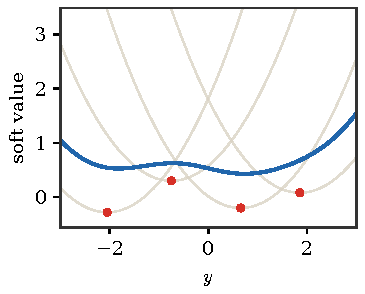
\includegraphics[width=.235\linewidth]{figures/sinkhorn-soft-c-transform-epsilon--eps-0p55.pdf} &
\index{soft!c-transform}% strictindex
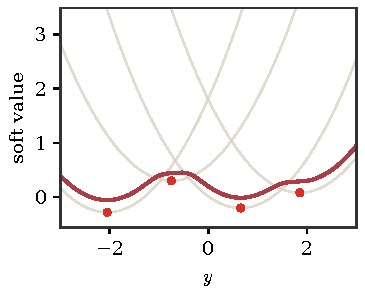
\includegraphics[width=.235\linewidth]{figures/sinkhorn-soft-c-transform-epsilon--eps-0p14.pdf} &
\index{c-transform}% strictindex
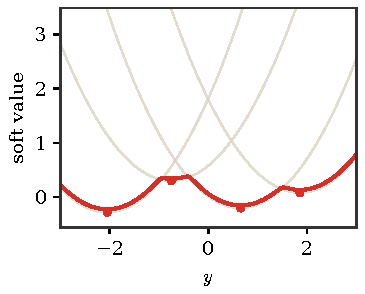
\includegraphics[width=.235\linewidth]{figures/sinkhorn-soft-c-transform-epsilon--eps-0p035.pdf} &
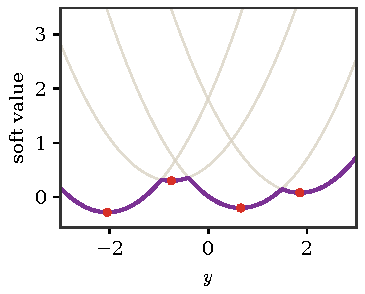
\includegraphics[width=.235\linewidth]{figures/sinkhorn-soft-c-transform-epsilon--hard.pdf}
\end{tabular}
\caption{\emph{Soft $c$-transforms for decreasing temperatures.} The hard transform is the lower envelope of shifted cost functions, while a positive $\epsilon$ replaces the pointwise minimum by a log-sum-exp soft minimum. As $\epsilon$ decreases, the soft transform sharpens and approaches the non-smooth hard envelope.}
\index{log-sum-exp}% strictindex
\index{soft!transform}% strictindex
\index{soft!minimum}% strictindex
\label{fig:sinkhorn-soft-c-transform-epsilon}
\end{figure}

\paragraph{Continuous dual and soft-transforms.}
\index{continuous!dual}% strictindex

For general, not necessarily discrete, measures $(\al,\be)$, the KL-regularized problem~\eqref{eq-entropic-generic} has the concave dual
\eql{\label{eq-dual-sinkh-cont}
	\MK_\c^\epsilon(\al,\be)
	=
	\usup{f\in\Cc(\Xx),\,g\in\Cc(\Yy)}
	\mathcal D_\epsilon(f,g),
}
where
\eql{\label{eq-dual-sinkhorn-objective}
	\mathcal D_\epsilon(f,g)
	\eqdef
	\int_{\Xx} f(x)\d\al(x)
	+
	\int_{\Yy} g(y)\d\be(y)
	-
	\epsilon
	\int_{\Xx\times\Yy}
	\pa{
		e^{\frac{f(x)+g(y)-c(x,y)}{\epsilon}}-1
	}
	\d\al(x)\d\be(y).
}
This is the smooth counterpart of the hard feasibility constraint $f\oplus g\leq c$ from the Kantorovich dual: violations are penalized exponentially and disappear in the limit $\epsilon\to0$.

The corresponding soft $c$-transforms are the exact block maximizers of this dual objective. They are the continuous log-integral counterparts of Definition~\ref{def-discrete-soft-c-transform}.

\begin{defn}[Continuous soft $c$-transforms]\label{def-continuous-soft-c-transform}
\index{soft!c-transform}% strictindex
\index{soft!transform}% strictindex
	For $f\in\Cc(\Xx)$ and $g\in\Cc(\Yy)$, define
	\begin{align}
		f^{c,\epsilon}(y)
		&\eqdef
		-\epsilon\log\!\left(
			\int_{\Xx}
			e^{\frac{f(x)-c(x,y)}{\epsilon}}\d\al(x)
		\right),
		\qquad y\in\Yy, \label{eq-soft-c-cont-f}\\
		g^{\bar c,\epsilon}(x)
		&\eqdef
		-\epsilon\log\!\left(
			\int_{\Yy}
			e^{\frac{g(y)-c(x,y)}{\epsilon}}\d\be(y)
		\right),
		\qquad x\in\Xx . \label{eq-soft-c-cont-g}
	\end{align}
\end{defn}
In the case of discrete measures, these formulas reduce to~\eqref{eq-discrete-soft-c-transforms}. The same calculus also gives the entropic semi-discrete problem: when one measure is discrete, one alternates between a finite-dimensional potential and an integral soft transform, often estimated stochastically.
\index{soft!transform}% strictindex
\index{semi-discrete!OT}% strictindex

\begin{prop}[Existence and uniqueness of entropic dual potentials]\label{prop-entropic-dual-potentials}
\index{dual!potential}% strictindex
	Assume that $\Xx=\supp(\al)$ and $\Yy=\supp(\be)$ are compact and that $c$ is continuous. The dual problem~\eqref{eq-dual-sinkh-cont} has solutions, and its set of solutions is
\index{dual!problem}% strictindex
	\[
		(f^\star+\lambda,g^\star-\lambda),
		\qquad \lambda\in\RR .
	\]
\end{prop}

\begin{proof}
	Normalize potentials by imposing $\int f\d\al=0$. Replacing any pair $(f,g)$ by the corresponding soft $c$-transforms does not decrease the dual objective, because each soft transform is the exact maximizer in one block variable. For transformed potentials, the oscillations are bounded by the oscillation of the cost:
\index{soft!c-transform}% strictindex
\index{soft!transform}% strictindex
	\[
		\norm{f}_V+\norm{g}_V
		\leq
		2(\sup c-\inf c).
	\]
	Moreover the modulus of continuity of the soft transforms is controlled by that of $c$; for instance
	\[
		\abs{g^{\bar c,\epsilon}(x)-g^{\bar c,\epsilon}(x')}
		\leq
		\sup_y\abs{c(x,y)-c(x',y)}.
	\]
	After normalization, maximizing sequences are therefore uniformly bounded and equicontinuous. Arzel\`a--Ascoli gives a uniformly converging subsequence, and continuity of~\eqref{eq-dual-sinkhorn-objective} gives a maximizer.

		For uniqueness, use strict convexity of
\index{strict!convexity}% strictindex
	\[
		H\mapsto \int e^{H/\epsilon}\d(\al\otimes\be)
	\]
		on the image of $(f,g)\mapsto H=f\oplus g-c$, modulo constants. If two optimal pairs exist, their midpoint is also optimal; strict convexity forces the two functions $f\oplus g$ to agree $\al\otimes\be$-almost everywhere. Full support and continuity then imply equality everywhere on $\Xx\times\Yy$, so $f-f'$ is constant and $g-g'$ is the opposite constant. Without replacing the ambient spaces by the marginal supports, uniqueness has this meaning only on those supports; values outside them do not enter the dual objective.
\end{proof}

\begin{rem}[Convexity properties of soft transforms]\label{rem-soft-transform-convexity}
\index{soft!transform}% strictindex
	The log-sum-exp part behaves like a smoothed maximum and preserves convexity. Since the soft transform takes the negative of this quantity after inserting the cost, it preserves the usual $c$-concavity structure. In particular, for the bilinear cost $c(x,y)=-\dotp{x}{y}$, the transform $f^{c,\epsilon}$ is concave for any $f$. Therefore, for the quadratic cost $c(x,y)=\norm{x-y}^2/2$, the optimal potentials have the form $f^\star(x)=\norm{x}^2/2-\phi^\star(x)$ and $g^\star(y)=\norm{y}^2/2-\psi^\star(y)$, where $\phi^\star$ and $\psi^\star$ are convex.
\index{log-sum-exp}% strictindex
\index{quadratic!cost}% strictindex
\index{c-concavity}% strictindex
\end{rem}

\paragraph{Neural dual solvers.}
\index{neural!dual solver}% strictindex
\index{neural!Sinkhorn solver}% strictindex
\index{input-convex neural network}% strictindex
\index{convex!neural network}% strictindex
The convex-potential structure of the preceding remark suggests a sample-based alternative to evaluating soft transforms on a grid or on all pairs of samples. For the bilinear cost \(c(x,y)=-\dotp{x}{y}\), the signs of the dual potentials are convex: writing \(\Phi=-f\) and \(\Psi=-g\), the zero-temperature constraint \(f(x)+g(y)\leq-\dotp{x}{y}\) becomes the Fenchel-type inequality
\[
	\Phi(x)+\Psi(y)\geq \dotp{x}{y}.
\]
For the quadratic cost this is the same statement after subtracting the quadratic terms, as in Remark~\ref{rem-soft-transform-convexity}. One can therefore maximize the continuous dual~\eqref{eq-dual-sinkhorn-objective} over parameterized convex potentials, estimating the integrals by stochastic samples.

A useful parameterization is given by input-convex neural networks (ICNNs)~\cite{amos2017input,makkuva2020optimal}. The construction mirrors elementary closure rules for convex functions: nonnegative linear combinations preserve convexity, composition with a convex nondecreasing scalar nonlinearity preserves convexity, and the ReLU \(r\mapsto\max(r,0)\) is both convex and nondecreasing. Thus a feed-forward network with nonnegative hidden-to-hidden weights and affine skip connections from the input defines a convex function of its input. This gives a flexible cone of convex trial potentials, although the finite-dimensional optimization over the network weights is not a convex optimization problem. Universal-approximation statements must also be read with this distinction in mind: max-affine functions are dense among continuous convex functions on compact convex sets, and ICNN-type architectures are designed to inherit this approximation principle. General ReLU universal approximation results, such as the width \(d+1\) theorem on compact subsets of \(\RR^d\)~\cite{hanin2019universal}, provide useful background but do not by themselves enforce convexity. In practice, neural dual solvers trade exact Sinkhorn scaling for amortized stochastic optimization of the dual potentials.
\index{neural!dual solver}% strictindex
\index{Fenchel inequality}% strictindex
\index{input-convex neural network}% strictindex
\index{convex!potential}% strictindex

\begin{rem}[Gaussian marginals]\label{rem-sinkhorn-gaussian-marginals}
\index{Gaussian!marginals}% strictindex
	For $c(x,y)=\norm{x-y}^2$ and Gaussian marginals, the soft transforms preserve quadratic functions, because products and convolutions of Gaussian functions remain Gaussian. Hence optimal entropic potentials are quadratic and the optimal entropic coupling is Gaussian. Section~\ref{sec-gaussian-sinkhorn} makes this finite-dimensional closure explicit.
\index{entropic!potential}% strictindex
\index{soft!transform}% strictindex
\end{rem}

%%%%%%%%%%%%%%%%%%%%%%%%%%%%%%%%%%%%%%%%%%%%%%%%%%%%%%%%%%%%%%%%%%%%%%%%%%%

\section{Marginal-Dependent Problems}
\index{marginal-dependent problem}% strictindex
\label{sec-sinkhorn-marginal-dependent}
\index{generalized Sinkhorn algorithm}% strictindex

The balanced Sinkhorn problem fixes both marginals exactly. Many nearby models instead optimize the transported marginals, but only through penalties or constraints applied separately to each marginal. The useful point, emphasized by the generalized scaling algorithms of Chizat, Peyr\'e, Schmitzer and Vialard~\cite{2016-chizat-sinkhorn}, is that entropic OT remains a diagonal-scaling problem whenever these marginal terms admit simple KL-proximal maps.
\index{KL proximal operator}% strictindex
\index{Sinkhorn!scaling}% strictindex
\index{unbalanced!OT}% strictindex

Let $\mathcal F$ and $\mathcal G$ be proper convex lower semicontinuous functionals on finite nonnegative measures on $\Xx$ and $\Yy$. The unregularized marginal-dependent transport problem is
\index{marginal-dependent problem}% strictindex
\begin{equation}\label{eq-marginal-dependent-unregularized-cont}
	\inf_{\pi\in\Mm_+(\Xx\times\Yy)}
	\int c(x,y)\d\pi(x,y)
	+
	\mathcal F(\pi_1)
	+
	\mathcal G(\pi_2),
\end{equation}
where $\pi_1=(\mathrm{p}_{\Xx})_\sharp\pi$ and $\pi_2=(\mathrm{p}_{\Yy})_\sharp\pi$ are the two marginals of $\pi$. Entropic regularization turns this problem into the scaling-friendly form
\begin{equation}\label{eq-marginal-dependent-cont}
	\inf_{\pi\in\Mm_+(\Xx\times\Yy)}
	\int c(x,y)\d\pi(x,y)
	+
	\mathcal F(\pi_1)
	+
	\mathcal G(\pi_2)
	+
	\epsilon\KL(\pi|\al\otimes\be),
\end{equation}
where $\al$ and $\be$ are reference measures. In this subsection, when the total mass of $\pi$ is not fixed, the KL term is understood in the generalized sense associated with $\varphi(s)=s\log s-s+1$. Thus, if $\lambda=\al\otimes\be$ and $\pi=\rho\lambda+\pi^\perp$ is the Lebesgue decomposition of $\pi$ with respect to $\lambda$, then
\[
	\KL(\pi|\lambda)
	=
	\int \bigl(\rho\log\rho-\rho+1\bigr)\d\lambda
\]
with value $+\infty$ when $\pi^\perp\ne0$. On probability couplings this coincides with the usual relative entropy.
\index{marginal!penalty}% strictindex
\index{relative!entropy}% strictindex
\index{Kullback-Leibler divergence}% strictindex

Several standard constructions fit this template. Balanced OT is recovered by taking $\mathcal F=\iota_{\{\al\}}$ and $\mathcal G=\iota_{\{\be\}}$. Unbalanced OT replaces these hard indicators by marginal divergences, as developed later in Section~\ref{sec-unbalanced}. An entropic JKO step fixes the first marginal to the previous iterate and puts the energy on the second marginal, for instance $\mathcal F=\iota_{\{\al_t\}}$ and $\mathcal G=E$, with cost $c/(2\tau)$; this is the static counterpart of the minimizing-movement schemes of Chapter~\ref{sec-wasserstein-gradient-flows}. Barycenters are the multi-coupling extension: several couplings share one unknown marginal and are treated by the generalized Sinkhorn updates of Section~\ref{sec-barycenters}.
\index{balanced OT}% strictindex
\index{JKO scheme}% strictindex
\index{Wasserstein!barycenter}% strictindex

In finite dimension, with reference weights satisfying $a_i,b_j>0$ and proper convex functions $\mathsf F:\RR_+^n\to\RR\cup\{+\infty\}$, $\mathsf G:\RR_+^m\to\RR\cup\{+\infty\}$, the entropic version becomes
\begin{equation}\label{eq-marginal-dependent-discrete}
	\inf_{\P\in\RR_+^{n\times m}}
	\dotp{\C}{\P}
	+
	\mathsf F(\P\ones_m)
	+
	\mathsf G(\transp{\P}\ones_n)
	+
	\epsilon\KLD(\P|\a\otimes\b).
\end{equation}
Equivalently, if $\K_{ij}=a_i b_j e^{-\C_{ij}/\epsilon}$, the terms involving $\C$ can be absorbed into the Gibbs reference and the problem is, up to the additive constant $\epsilon\sum_{i,j}(a_i b_j-\K_{ij})$,
\[
	\inf_{\P\geq0}
	\mathsf F(\P\ones_m)
	+
	\mathsf G(\transp{\P}\ones_n)
	+
	\epsilon\KLD(\P|\K).
\]
\index{Gibbs!kernel}% strictindex
\index{KL!projection}% strictindex

\begin{prop}[Dual and scaling for marginal penalties]\label{prop-marginal-dependent-dual-scaling}
\index{marginal-dependent problem}% strictindex
Assume $a_i,b_j>0$, $\epsilon>0$, and a Fenchel qualification condition, for instance the existence of a matrix $\P>0$ such that $\P\ones_m$ and $\transp{\P}\ones_n$ belong to the relative interiors of $\dom(\mathsf F)$ and $\dom(\mathsf G)$. The Fenchel dual of~\eqref{eq-marginal-dependent-discrete} is
\begin{equation}\label{eq-marginal-dependent-dual}
	\sup_{\fD\in\RR^n,\gD\in\RR^m}
	-
	\mathsf F^*(-\fD)
	-
	\mathsf G^*(-\gD)
	-
	\epsilon\sum_{i,j}a_i b_j
	\left[
		\exp\left(\frac{\fD_i+\gD_j-\C_{ij}}{\epsilon}\right)-1
	\right].
\end{equation}
Equivalently, up to the additive constant $\epsilon\sum_{i,j}a_i b_j$, the last term is
\[
	-
	\epsilon\sum_{i,j}\K_{ij}
	\exp\left(\frac{\fD_i+\gD_j}{\epsilon}\right).
\]
If $\uD=e^{\fD/\epsilon}$ and $\vD=e^{\gD/\epsilon}$, exact block ascent in the two dual variables is the generalized Sinkhorn cycle
\begin{equation}\label{eq-generalized-sinkhorn-kl-prox}
\begin{aligned}
	r &\leftarrow \prox_{\mathsf F/\epsilon}^{\KLD}(\K\vD),
	&\qquad
	\uD &\leftarrow r\oslash(\K\vD),\\
	s &\leftarrow \prox_{\mathsf G/\epsilon}^{\KLD}(\transp{\K}\uD),
	&\qquad
	\vD &\leftarrow s\oslash(\transp{\K}\uD),\\
	\P&=\diag(\uD)\K\diag(\vD),
\end{aligned}
\end{equation}
where divisions are entrywise and
\begin{equation}\label{eq-kl-prox-marginal}
	\prox_{\mathsf h}^{\KLD}(z)
	\eqdef
	\uargmin{r\in\RR_+^d}
	\mathsf h(r)+\KLD(r|z).
\end{equation}
In particular, $\prox_{\mathsf F/\epsilon}^{\KLD}(z)$ is the minimizer of $\mathsf F(r)+\epsilon\KLD(r|z)$.
\end{prop}

\begin{proof}
Introduce independent variables $r$ and $s$ for the two marginals and use dual variables $\fD,\gD$ for the constraints $r=\P\ones_m$ and $s=\transp{\P}\ones_n$. The Lagrangian contains
\[
	\mathsf F(r)+\dotp{\fD}{r}
	+
	\mathsf G(s)+\dotp{\gD}{s}
	+
	\dotp{\C}{\P}
	+
	\epsilon\KLD(\P|\a\otimes\b)
	-
	\dotp{\fD\oplus\gD}{\P}.
\]
Minimizing over $r$ and $s$ gives $-\mathsf F^*(-\fD)$ and $-\mathsf G^*(-\gD)$. For each scalar entry, the convex conjugate of $p\mapsto \C_{ij}p+\epsilon(p\log(p/(a_i b_j))-p+a_i b_j)$ is $q\mapsto \epsilon a_i b_j(e^{(q-\C_{ij})/\epsilon}-1)$. Minimizing over $\P$ with $q=\fD_i+\gD_j$ gives~\eqref{eq-marginal-dependent-dual}.
\index{marginal-dependent problem}% strictindex

For the scaling form, fix $\vD>0$, set $\widetilde{\K}=\K\diag(\vD)$ and $z=\widetilde{\K}\ones_m=\K\vD$. Updating the row scaling means looking for $\P=\diag(\uD)\widetilde{\K}$, so its row marginal is $r=\P\ones_m=\uD\odot z$. The row-wise chain rule gives
\[
	\KLD(\diag(\uD)\widetilde{\K}|\widetilde{\K})
	=
	\sum_i \bigl(r_i\log(r_i/z_i)-r_i+z_i\bigr)
	=
	\KLD(r|z).
\]
Thus exact optimization of this block is equivalent to minimizing $\mathsf F(r)+\epsilon\KLD(r|z)$ over $r\geq0$, hence $r=\prox_{\mathsf F/\epsilon}^{\KLD}(z)$ and $\uD=r\oslash z$. The column update is identical with $w=\transp{\K}\uD$.
\end{proof}
\index{Fenchel duality}% strictindex
\index{dual!Sinkhorn}% strictindex
\index{KL!proximal map}% strictindex
\index{dual!ascent}% strictindex
\index{multiplicative scaling}% strictindex

When $\mathsf F=\iota_{\{\a\}}$ and $\mathsf G=\iota_{\{\b\}}$, the first two dual terms are $\dotp{\fD}{\a}+\dotp{\gD}{\b}$, and one recovers the usual entropic dual~\eqref{eq-dual-sinkhorn-objective}. The classical Sinkhorn update is the special case in which the KL proximal maps return the prescribed marginals $\a$ and $\b$.

\begin{alg}[Generalized Sinkhorn for marginal penalties]\label{alg-generalized-sinkhorn-marginal-penalties}
\index{generalized Sinkhorn algorithm}% strictindex
\textbf{Input:} Reference weights $\a,\b$, cost $\C$, convex marginal penalties $\mathsf F,\mathsf G$, regularization $\epsilon>0$, tolerance $\mathrm{tol}$.

\textbf{Output:} Coupling $\P$ and optimized marginals $r=\P\ones_m$, $s=\transp{\P}\ones_n$.

\textbf{Set} $\K_{ij}=a_i b_j e^{-\C_{ij}/\epsilon}$.

\textbf{Initialize:} $\uD=\ones_n$, $\vD=\ones_m$, $\eta=+\infty$.

\textbf{While} $\eta>\mathrm{tol}$ \textbf{do}:
\begin{algblock}
\textbf{Store} $\uD_{\mathrm{old}}=\uD$ and $\vD_{\mathrm{old}}=\vD$.

\textbf{Set} $z=\K\vD$.

\textbf{Compute} $r=\prox_{\mathsf F/\epsilon}^{\KLD}(z)$.

\textbf{Set} $\uD=r\oslash z$.

\textbf{Set} $w=\transp{\K}\uD$.

\textbf{Compute} $s=\prox_{\mathsf G/\epsilon}^{\KLD}(w)$.

\textbf{Set} $\vD=s\oslash w$.

\textbf{Set} $\eta=\max\{\norm{\uD-\uD_{\mathrm{old}}}_\infty,\norm{\vD-\vD_{\mathrm{old}}}_\infty\}$.
\end{algblock}
\algreturnskip
\textbf{Return} $\P=\diag(\uD)\K\diag(\vD)$, $r=\P\ones_m$, and $s=\transp{\P}\ones_n$.
\end{alg}

The usefulness of this formulation is that many KL-proximal maps are explicit.
\index{KL proximal operator}% strictindex
\index{KL!proximal map}% strictindex
\begin{itemize}
	\item \textbf{Hard marginal constraint.} If $\mathsf F=\iota_{\{\a\}}$, then $\prox_{\mathsf F/\epsilon}^{\KLD}(z)=\a$.
	\item \textbf{KL marginal relaxation.} If $\mathsf F(r)=\tau\KLD(r|\a)$ with $\tau>0$, then, coordinatewise,
	\[
		\prox_{\mathsf F/\epsilon}^{\KLD}(z)
		=
		z^{\epsilon/(\tau+\epsilon)}\odot \a^{\tau/(\tau+\epsilon)},
	\]
	and the scaling update becomes $\uD\leftarrow(\a\oslash z)^{\tau/(\tau+\epsilon)}$, the damped scaling of unbalanced Sinkhorn.
	\item \textbf{Pointwise bounds.} If $\mathsf F=\iota_{\{\ell\leq r\leq u\}}$, then the proximal map is the coordinatewise clipping $\prox_{\mathsf F/\epsilon}^{\KLD}(z)_i=\min\{u_i,\max\{\ell_i,z_i\}\}$.
	\item \textbf{Total-variation marginal relaxation.} If $\mathsf F(r)=\tau\norm{r-\a}_1$ and $\lambda=\tau/\epsilon$, then the proximal map is coordinatewise
	\[
		\prox_{\mathsf F/\epsilon}^{\KLD}(z)_i
		=
		\begin{cases}
		z_i e^{\lambda}, & z_i<a_i e^{-\lambda},\\
		a_i, & a_i e^{-\lambda}\leq z_i\leq a_i e^{\lambda},\\
		z_i e^{-\lambda}, & z_i>a_i e^{\lambda}.
		\end{cases}
	\]
	\item \textbf{Fixed total mass.} If $\mathsf F=\iota_{\{\dotp{r}{\ones}=m\}}$, then $\prox_{\mathsf F/\epsilon}^{\KLD}(z)=m z/\dotp{z}{\ones}$.
\end{itemize}
These examples explain why generalized Sinkhorn algorithms remain practical: the expensive operation is still multiplication by $\K$ or $\transp{\K}$, while the model-specific part is a low-dimensional KL-proximal update on a marginal.
\index{KL proximal operator}% strictindex
\index{marginal!penalty}% strictindex
\index{unbalanced!Sinkhorn}% strictindex

%%%%%%%%%%%%%%%%%%%%%%%%%%%%%%%%%%%%%%%%%%%%%%%%%%%%%%%%%%%%%%%%%%%%%%%%%%%
\section{Heat Kernels and Hopf--Cole Transforms}
\index{heat kernel}% strictindex
\index{Hopf-Cole transform}% strictindex
\index{geodesics in heat}% strictindex
\label{sec-sinkhorn-heat-hopf-cole}

The Gaussian kernel used by Sinkhorn is also the Euclidean heat kernel. This viewpoint clarifies when entropic OT admits fast grid and surface implementations, and it places soft minima and Hopf--Cole transforms in the same heat-kernel calculus.

\paragraph{Geodesics in heat.}
\index{Varadhan formula}% strictindex
\index{Laplace-Beltrami operator}% strictindex

On $\RR^d$, the heat kernel for $\partial_t u=\Delta u$ is
\index{heat kernel}% strictindex
\[
	h_t(x,y)=(4\pi t)^{-d/2}\exp\!\left(-\frac{\norm{x-y}^2}{4t}\right).
\]
For the quadratic cost $c(x,y)=\norm{x-y}^2$, the Gibbs kernel used by Sinkhorn satisfies
\[
	\K_\epsilon(x,y)
	\eqdef e^{-\norm{x-y}^2/\epsilon}
	=
	(\pi\epsilon)^{d/2}h_{\epsilon/4}(x,y).
\]
The scalar factor is absorbed by the Sinkhorn scalings and therefore does not change the optimal coupling. On a Riemannian manifold or surface $M$, let $L=-\Delta_M$ and replace the dense Gibbs kernel by the intrinsic heat operator $\mathsf H_\epsilon\eqdef e^{-(\epsilon/4)L}$. For histograms on the same discretized domain, the scaling steps become
\[
	\uD^{(\ell+1)}=\a\oslash\bigl(\mathsf H_\epsilon\vD^{(\ell)}\bigr),
	\qquad
	\vD^{(\ell+1)}=\b\oslash\bigl(\mathsf H_\epsilon^\top\uD^{(\ell+1)}\bigr).
\]
Here $\mathsf H_\epsilon$ includes quadrature weights and $\mathsf H_\epsilon^\top$ is its discrete adjoint; they coincide in a symmetric mass-normalized discretization. Thus heat diffusion fits Sinkhorn at its only expensive operation: multiplication by the Gibbs kernel. Equivalently, it uses the effective cost $c_\epsilon(x,y)\eqdef-\epsilon\log h_{\epsilon/4}(x,y)$, and Varadhan's formula gives
\[
	c_\epsilon(x,y)\longrightarrow d_M(x,y)^2
	\qquad (\epsilon\downarrow0).
\]
Hence convolutional Sinkhorn recovers the squared geodesic ground cost at small temperature without computing all pairwise geodesic distances~\cite{varadhan-1967,2015-solomon-siggraph}. The same asymptotic relation underlies geodesics-in-heat distance estimation~\cite{Crane2013}.

The heat operator can be applied through shifted-Laplacian solves,
\[
	\mathsf H_\epsilon
	=
	\lim_{q\to\infty}
	\left(I+\frac{\epsilon}{4q}L\right)^{-q}.
\]
On a triangulated surface or image grid, replace $L$ by a sparse positive semidefinite Laplacian $L_h$ and set $A_{\epsilon,q}\eqdef I+\epsilon L_h/(4q)$. For fixed $(\epsilon,q)$, a sparse Cholesky factorization $A_{\epsilon,q}=RR^\top$ is computed once. Each application of $\mathsf H_\epsilon$ is then approximated by $q$ successive solves with $A_{\epsilon,q}$, and the same factorization is reused throughout Sinkhorn's iterations~\cite{2015-solomon-siggraph}. This avoids a dense kernel and all-pairs geodesic distances. The diffusion length is of order $\sqrt\epsilon$ and must be resolved by the mesh; taking $\epsilon$ smaller than the squared grid spacing produces metrication and discretization artifacts.
\index{heat kernel}% strictindex
\index{mesh size}% strictindex
\index{discrete!Laplacian}% strictindex
\index{resolvent}% strictindex
\index{geodesic!distance}% strictindex

Figure~\ref{fig:sinkhorn-geodesics-in-heat} compares the exact distance to a non-convex source curve with heat-kernel and shifted-Laplacian approximations at several smoothing scales.

\begin{figure}[H]
\centering
\setlength{\tabcolsep}{2pt}
\begin{tabular}{@{}cccc@{}}
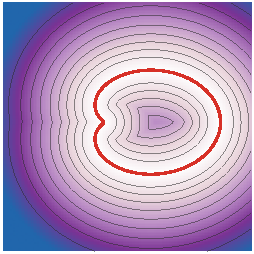
\includegraphics[width=.235\linewidth]{figures/sinkhorn-geodesics-in-heat--exact.pdf} &
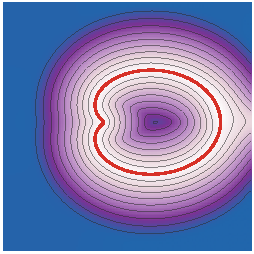
\includegraphics[width=.235\linewidth]{figures/sinkhorn-geodesics-in-heat--epsilon-small.pdf} &
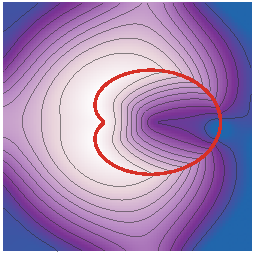
\includegraphics[width=.235\linewidth]{figures/sinkhorn-geodesics-in-heat--epsilon-medium.pdf} &
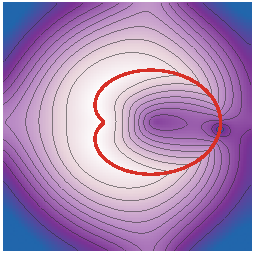
\includegraphics[width=.235\linewidth]{figures/sinkhorn-geodesics-in-heat--epsilon-large.pdf} \\[-.1em]
\small exact distance &
\small small $\epsilon$ &
\small medium $\epsilon$ &
\small larger $\epsilon$
\end{tabular}
\caption{\emph{Geodesics-in-heat approximation of the distance to a dense red non-convex source curve on a two-dimensional grid.} The first panel shows the exact Euclidean distance to the curve. The other panels diffuse a narrow band by the one-step approximation $(I+\epsilon L_h/4)^{-1}$ with Neumann boundary conditions, then recover a distance by the normalized-gradient Poisson solve. Increasing the Sinkhorn temperature $\epsilon$ suppresses unresolved grid-scale artifacts but progressively rounds the non-convex level-set geometry.}
\index{geodesics in heat}% strictindex
\index{Poisson equation}% strictindex
\label{fig:sinkhorn-geodesics-in-heat}
\end{figure}


\paragraph{Soft Hopf--Lax and Hopf--Cole.}
\index{Hopf-Lax formula}% strictindex
\index{Hopf-Cole transform}% strictindex
\index{log-sum-exp}% strictindex

The Hopf--Lax formula is the Hamilton--Jacobi incarnation of the hard $c$-transform. We use the normalized quadratic cost
\[
	c(x,y)=\frac12\norm{x-y}^2,
\]
so that the Hopf--Lax operator applied to an initial datum $h$ is precisely
\[
	(-h)^{\bar c}(x)=\inf_y\left\{h(y)+\frac12\norm{x-y}^2\right\},
\]
where the sign only reflects the convention of Definition~\ref{def-c-transform}. This is the usual Hopf--Lax formula for the Hamiltonian $\norm{p}^2/2$~\cite{evans2010pde,Villani09}; other quadratic scalings amount to multiplying the cost by a constant. In the present entropic setting, the parameter of interest is instead the temperature $\epsilon$.

The soft version replaces the infimum by a log-sum-exp soft minimum. In the notation of Definition~\ref{def-continuous-soft-c-transform}, and using Lebesgue measure on $\RR^d$,
\begin{equation}\label{eq-soft-hopf-lax-heat}
	(-h)^{\bar c,\epsilon}(x)
	=
	-\epsilon\log
	\int
	\exp\!\left(
	-\frac{h(y)+\norm{x-y}^2/2}{\epsilon}
	\right)\d y .
	\end{equation}
This is a soft $c$-transform of the function $-h$, and Laplace's principle gives $(-h)^{\bar c,\epsilon}\to(-h)^{\bar c}$ as $\epsilon\to0$ under the usual compactness assumptions on near-minimizers. The same formula is also a heat-kernel formula. If
\[
	G_\epsilon(z)\eqdef (2\pi\epsilon)^{-d/2}\exp\!\left(-\frac{\norm{z}^2}{2\epsilon}\right)
\]
is the normalized Gaussian kernel with covariance $\epsilon\Id$, then~\eqref{eq-soft-hopf-lax-heat} is exactly
\begin{equation}\label{eq-soft-c-transform-gaussian-convolution}
	(-h)^{\bar c,\epsilon}(x)
	=
	-\epsilon\log\Big(G_\epsilon\ast e^{-h/\epsilon}\Big)(x)
	-\frac{\epsilon d}{2}\log(2\pi\epsilon).
\end{equation}
Thus a soft quadratic $c$-transform is a Gaussian convolution followed by a logarithm, up to an explicit additive constant independent of $x$. This is the bridge between soft-minimum operators, heat kernels and entropic transport potentials.
\index{heat kernel}% strictindex
\index{Gaussian!convolution}% strictindex
\index{soft!c-transform}% strictindex

\begin{prop}[Soft quadratic $c$-transform and Legendre approximation]\label{prop-soft-legendre-convolution}
\index{Legendre-Fenchel transform}% strictindex
\index{fast Legendre transform}% strictindex
Let $f:\RR^d\to\RR\cup\{+\infty\}$ be such that the integrals below are finite, and introduce the quadratic shift
\[
	\mathsf S f(y)\eqdef f(y)-\frac12\norm{y}^2.
\]
For $\epsilon>0$, define the soft conjugate by applying the soft $\bar c$-transform to the shifted function:
\begin{equation}\label{eq-soft-legendre-definition}
	f^{*,\epsilon}(p)
	\eqdef
	\frac12\norm{p}^2-\big(-\mathsf S f\big)^{\bar c,\epsilon}(p).
\end{equation}
Then
\begin{equation}\label{eq-soft-legendre-logsumexp}
	f^{*,\epsilon}(p)
	=
	\epsilon\log\int_{\RR^d}
	\exp\!\left(\frac{\dotp{p}{y}-f(y)}{\epsilon}\right)\d y,
\end{equation}
and equivalently
\begin{equation}\label{eq-soft-legendre-convolution}
	f^{*,\epsilon}(p)
	=
	\frac12\norm{p}^2
	+\epsilon\log\Big(G_\epsilon\ast e^{-\mathsf S f/\epsilon}\Big)(p)
	+\frac{\epsilon d}{2}\log(2\pi\epsilon).
\end{equation}
If, for instance, $f$ is proper, lower semicontinuous and superlinear, then $f^{*,\epsilon}(p)\to f^*(p)$ for every $p$ as $\epsilon\to0$.
\end{prop}

\begin{proof}
The hard identity follows by completing the square:
\[
	\inf_y\left\{\mathsf S f(y)+\frac12\norm{p-y}^2\right\}
	=
	\frac12\norm{p}^2-
	\sup_y\{\dotp{p}{y}-f(y)\}
	=
	\frac12\norm{p}^2-f^*(p).
\]
This explains the shift: it turns the Legendre--Fenchel transform into a quadratic $\bar c$-transform. Replacing the hard transform by its soft version gives~\eqref{eq-soft-legendre-definition}. Expanding the square in~\eqref{eq-soft-hopf-lax-heat} with the function $\mathsf S f$ gives
\[
	\exp\!\left(-\frac{\mathsf S f(y)+\norm{p-y}^2/2}{\epsilon}\right)
	=
	\exp\!\left(-\frac{\norm{p}^2}{2\epsilon}\right)
	\exp\!\left(\frac{\dotp{p}{y}-f(y)}{\epsilon}\right),
\]
which proves~\eqref{eq-soft-legendre-logsumexp}. Formula~\eqref{eq-soft-legendre-convolution} is the Gaussian-convolution identity~\eqref{eq-soft-c-transform-gaussian-convolution} applied to $\mathsf S f$. Under the stated superlinearity assumption, the functions $y\mapsto\dotp{p}{y}-f(y)$ have compact upper level sets, so Laplace's principle applied to~\eqref{eq-soft-legendre-logsumexp} gives the convergence to $f^*(p)$.
\end{proof}

\begin{rem}[Fast soft Legendre--Fenchel transforms]\label{rem-soft-legendre-fft}
\index{Legendre-Fenchel transform}% strictindex
\index{fast Legendre transform}% strictindex
\index{FFT}% strictindex
\index{Gaussian!convolution}% strictindex
	Proposition~\ref{prop-soft-legendre-convolution} gives a computational recipe for a smoothed Legendre--Fenchel transform. On a periodic, or sufficiently padded, grid, the term $G_\epsilon\ast e^{-\mathsf S f/\epsilon}$ in~\eqref{eq-soft-legendre-convolution} is a Gaussian convolution. It can therefore be evaluated in $O(N\log N)$ operations for $N$ grid samples using an FFT. This is not an exact hard discrete Legendre transform, but a regularized approximation whose zero-temperature limit recovers the hard transform by Laplace's principle. Exact discrete conjugation and lower-envelope algorithms exploit convex-analytic and computational-geometry structure instead; see Lucet's survey of computational convex analysis and the distance-transform algorithm of Felzenszwalb and Huttenlocher~\cite{Lucet2010ComputationalConvexAnalysis,FelzenszwalbHuttenlocher2012DistanceTransforms}.

	The convolutional route is nevertheless delicate when $\epsilon$ is small. In fixed precision, the factors $e^{-f/\epsilon}$ or $e^{-\mathsf S f/\epsilon}$ can underflow or overflow, and the logarithm can amplify small relative convolution errors. Practical implementations therefore use shifts, log-domain evaluations, or stabilized FFT convolutions. In dimension $d$, one can also use the same separability of the Gaussian kernel as in grid Sinkhorn: direct one-dimensional passes give the tensor-product cost~\eqref{eq-separable-gaussian-half-step}, namely $O(d\,N^{1+1/d})$, while FFT convolutions provide an additional acceleration when boundary conditions and conditioning permit it.
\end{rem}

Figure~\ref{fig:sinkhorn-soft-biconjugates} illustrates the biconjugation viewpoint directly. The red curve is the hard lower convex envelope $f^{**}$, while the blue curves are smoother finite-temperature biconjugates. The two examples show that the same mechanism convexifies both a simple double-well profile and a quadratic oscillatory landscape.
\index{Legendre-Fenchel transform}% strictindex
\index{convex!envelope}% strictindex

\begin{figure}[H]
\centering
\setlength{\tabcolsep}{2.5pt}
\begin{tabular}{@{}cc@{}}
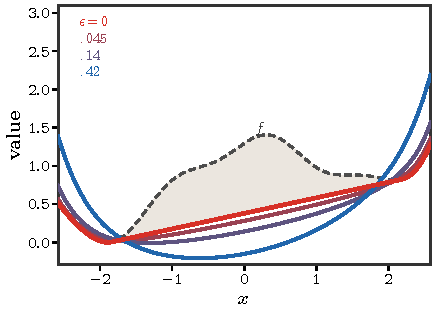
\includegraphics[width=.47\linewidth]{figures/sinkhorn-hopf-cole-transform--biconjugate-simple.pdf} &
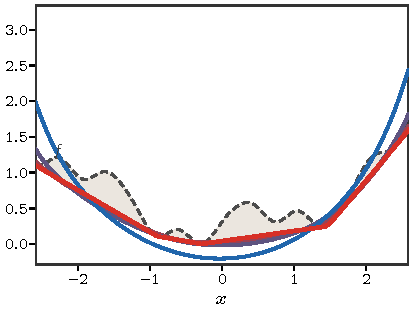
\includegraphics[width=.47\linewidth]{figures/sinkhorn-hopf-cole-transform--biconjugate-oscillatory.pdf} \\[-.1em]
\small smooth double well &
\small quadratic oscillatory profile
\end{tabular}
\caption{\emph{Soft Legendre biconjugates as approximations of lower convex envelopes.} In each panel, the dashed gray curve is a non-convex function $f$, the red curve is the hard biconjugate $f^{**}$, and the purple-to-blue curves show $(f^{*,\epsilon})^{*,\epsilon}$ for increasing $\epsilon$. The pale gray area marks the part of $f$ lying above its convex envelope, which is progressively filled in by the soft convexification.}
\label{fig:sinkhorn-soft-biconjugates}
\end{figure}

The nonlinear PDEs are linearized by the Hopf--Cole transform. With the same temperature normalization, the change of variables $u_s=e^{-\phi_s/\epsilon}$ converts the viscous Hamilton--Jacobi equation
\index{Hopf-Cole transform}% strictindex
\[
	\partial_s\phi_s+\frac12\norm{\nabla\phi_s}^2=\frac{\epsilon}{2}\Delta\phi_s,
\]
into the linear heat equation $\partial_su_s=(\epsilon/2)\Delta u_s$. Conversely, starting from a positive heat solution $u_s$ and setting $\phi_s=-\epsilon\log u_s$ gives a Hamilton--Jacobi solution, while
$v_s=\nabla\phi_s=-\epsilon\nabla\log u_s$ solves the gradient viscous Burgers equation
\[
	\partial_s v_s+(v_s\cdot\nabla)v_s=\frac{\epsilon}{2}\Delta v_s .
\]
Thus nonlinear Hamilton--Jacobi/Burgers dynamics can be computed through a Laplacian-generated heat flow followed by a logarithmic change of variables. In one dimension this is the classical Cole--Hopf transform for viscous Burgers; in higher dimension this scalar reduction applies to irrotational velocity fields. Figure~\ref{fig:sinkhorn-hopf-cole-transform} starts from a Gaussian velocity bump, whose inviscid evolution would form a shock on its decreasing flank, and shows how the viscosity parameter $\epsilon/2$ regularizes this steepening. Together with Figure~\ref{fig:sinkhorn-soft-biconjugates}, it gives the two complementary viewpoints behind soft-minimum formulas, Gaussian convolution and entropic transport potentials.
\index{Burgers equation}% strictindex
\index{Hamilton-Jacobi equation}% strictindex
\index{heat equation}% strictindex
\index{Hopf-Lax formula}% strictindex

\begin{figure}[H]
\centering
\setlength{\tabcolsep}{2.5pt}
\begin{tabular}{@{}ccc@{}}
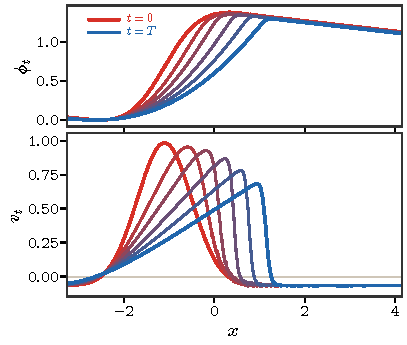
\includegraphics[width=.318\linewidth]{figures/sinkhorn-hopf-cole-transform--burgers-epsilon-small.pdf} &
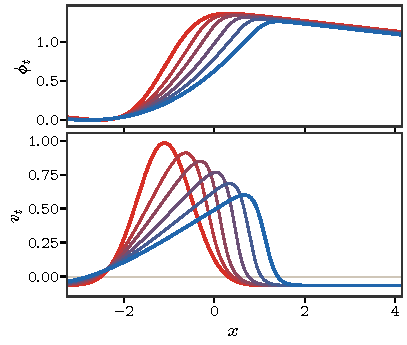
\includegraphics[width=.318\linewidth]{figures/sinkhorn-hopf-cole-transform--burgers-epsilon-medium.pdf} &
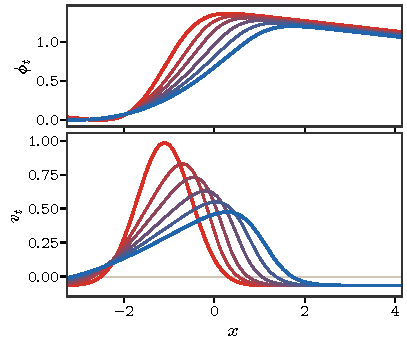
\includegraphics[width=.318\linewidth]{figures/sinkhorn-hopf-cole-transform--burgers-epsilon-large.pdf} \\[-.1em]
\small $\epsilon=.038$ &
\small $\epsilon=.10$ &
\small $\epsilon=.24$
\end{tabular}
\caption{\emph{Hopf--Cole numerics for viscous Hamilton--Jacobi and Burgers dynamics in one dimension.} Each panel fixes $\epsilon$ and evolves the same initial Gaussian-shaped Burgers velocity. The upper curves show the potential $\phi_t$ obtained from the heat solution by $\phi_t=-\epsilon\log u_t$, while the lower curves show the Burgers velocity $v_t=\partial_x\phi_t=-\epsilon\,\partial_x\log u_t$. Colors encode time from red to blue; small $\epsilon$ lets the Gaussian bump develop a sharp shock-like front, while larger $\epsilon$ gives stronger heat smoothing and viscous damping.}
\index{Hopf-Cole transform}% strictindex
\index{Burgers equation}% strictindex
\label{fig:sinkhorn-hopf-cole-transform}
\end{figure}


%%%%%%%%%%%%%%%%%%%%%%%%%%%%%%%%%%%%%%%%%%%%%%%%%%%%%%%%%%%%%%%%%%%%%%%%%%%
\section{Other Convex Regularizers}
\index{convex!regularizer}% strictindex
\label{sec-sinkhorn-other-regularizers}

KL regularization is the case that leads to multiplicative Sinkhorn scalings. Replacing the KL divergence by another density-ratio penalty keeps the same transport constraints but changes the scalar law linking the optimal density to the dual potentials.
\index{Sinkhorn!scaling}% strictindex
\index{dual!potential}% strictindex
\index{density!ratio}% strictindex

\paragraph{$\phi$-divergence regularization.}

The primal and dual problems retain the same transport constraints, but the exponential Gibbs law is replaced by the derivative of a general convex conjugate.

Let $\phi$ be an entropy function in the sense of Definition~\ref{def_entropy}, and recall the $\phi$-divergence $\Divergm_\phi$ from Definition~\ref{def_divergence}. For $\epsilon>0$, define the $\phi$-regularized transport value
\index{entropy!function}% strictindex
\index{phi-divergence}% strictindex
\eql{\label{eq-phi-regularized-ot}
\index{phi-divergence regularized OT}% strictindex
	\MK_{\c,\phi}^{\epsilon}(\al,\be)
	\eqdef
	\umin{\pi\in\Couplings(\al,\be)}
	\int_{\Xx\times\Yy} c(x,y)\d\pi(x,y)
	+
	\epsilon\Divergm_\phi(\pi|\al\otimes\be).
}

\begin{prop}[Dual and density law for $\phi$-regularized OT]\label{prop-phi-regularized-ot-dual}
\index{phi-divergence regularized OT}% strictindex
	Assume that the Fenchel--Rockafellar qualification condition holds; for example, let the spaces be compact, let $c$ be continuous, and assume that the product coupling belongs to the continuity domain of the divergence term. Then
\index{duality!Fenchel-Rockafellar}% strictindex
\index{Fenchel duality}% strictindex
	\eql{\label{eq-phi-regularized-ot-dual}
		\MK_{\c,\phi}^{\epsilon}(\al,\be)
		=
		\usup{f\in\Cc(\Xx),\,g\in\Cc(\Yy)}
		\int f\d\al+\int g\d\be
		-
		\epsilon
		\int
		\phi^*\!\left(\frac{f(x)+g(y)-c(x,y)}{\epsilon}\right)
		\d\al(x)\d\be(y).
	}
	If an optimal plan is absolutely continuous, with density $r^\star=\frac{\d\pi^\star}{\d(\al\otimes\be)}$, and $(f^\star,g^\star)$ are optimal potentials, then
\index{optimal plan}% strictindex
	\eql{\label{eq-phi-regularized-ot-density-law}
		\frac{f^\star(x)+g^\star(y)-c(x,y)}{\epsilon}
		\in
		\partial\phi(r^\star(x,y))
		\qquad
		\al\otimes\be\text{-a.e.}
	}
	In the smooth interior this reads
	\[
		r^\star(x,y)
		=
		(\phi')^{-1}
		\!\left(\frac{f^\star(x)+g^\star(y)-c(x,y)}{\epsilon}\right).
	\]
\end{prop}

\begin{proof}
	Introduce dual variables $(f,g)$ for the two marginal constraints. For fixed $(f,g)$, the minimization over $\pi$ gives
\index{marginal!constraint}% strictindex
	\[
		\int f\d\al+\int g\d\be
		+
		\inf_{\pi\in\Mm_+(\Xx\times\Yy)}
		\left\{
		\int\big(c-(f\oplus g)\big)\d\pi
		+
		\epsilon\Divergm_\phi(\pi|\al\otimes\be)
		\right\}.
	\]
	Using the Legendre formula~\eqref{eq-legendre} for the convex functional $\Divergm_\phi(\cdot|\al\otimes\be)$, the infimum equals
\index{convex!function}% strictindex
	\[
		-\epsilon
		\int
		\phi^*\!\left(\frac{f(x)+g(y)-c(x,y)}{\epsilon}\right)
		\d\al(x)\d\be(y),
	\]
	which gives~\eqref{eq-phi-regularized-ot-dual}. Equality in the Fenchel inequality is equivalent to the subgradient inclusion
\index{phi-divergence regularized OT}% strictindex
	\[
		\frac{f^\star\oplus g^\star-c}{\epsilon}
		\in
		\partial\phi(r^\star),
	\]
	and inversion of $\phi'$ gives the density law when $\phi$ is differentiable and the optimizer is in the interior of its domain.
\end{proof}

For the KL entropy $\phi(r)=r\log r-r+1$, one has $\phi^*(s)=e^s-1$, and~\eqref{eq-phi-regularized-ot-dual} reduces exactly to the continuous Sinkhorn dual~\eqref{eq-dual-sinkhorn-objective}. Other choices replace the exponential density law by another scalar transfer function:
\index{Sinkhorn!dual}% strictindex
\index{continuous!Sinkhorn dual}% strictindex
\index{phi-divergence regularized OT}% strictindex
\[
\begin{array}{lll}
	\phi(r)=r\log r-r+1 &\Rightarrow& r^\star=e^s,\\[.25em]
	\phi(r)=r-\log r-1 &\Rightarrow& r^\star=(1-s)^{-1}\quad (s<1),\\[.25em]
	\phi(r)=\frac12(r-1)^2 &\Rightarrow& r^\star=(1+s)_+,
\end{array}
\qquad
s\eqdef\frac{f^\star\oplus g^\star-c}{\epsilon}.
\]

\paragraph{Bregman-divergence regularization.}
\index{Bregman!regularization}% strictindex
\index{phi-divergence}% strictindex

The previous construction regularizes OT by a density-ratio divergence. This differs from using a Bregman divergence generated by a convex functional on the space of measures.
\index{convex!function}% strictindex
\index{Bregman!divergence}% strictindex
\index{reference!measure}% strictindex
\index{density!ratio}% strictindex

\begin{defn}[Measure Bregman divergence]\label{def-measure-bregman-divergence}
\index{first variation}% strictindex
	If $\Phi$ is a differentiable convex functional on a convex class of nonnegative measures and $\xi$ is a reference measure in its domain, the measure Bregman divergence generated by $\Phi$ is
	\begin{equation}\label{eq-measure-bregman-divergence}
		B_\Phi(\pi|\xi)
		\eqdef
		\Phi(\pi)-\Phi(\xi)
		-
		\int \delta\Phi(\xi)\d(\pi-\xi),
	\end{equation}
	where $\delta\Phi(\xi)$ is the first variation in the sense of Definition~\ref{def-first-variation}, and the formula is understood whenever the right-hand side is well-defined.
\end{defn}
In finite dimension this reduces to Definition~\ref{def-bregman-divergence}.
\index{first variation}% strictindex
\index{Wasserstein!gradient flow}% strictindex
\index{Bregman!divergence}% strictindex
\index{density!ratio}% strictindex

\begin{prop}[Dual and density law for Bregman-regularized OT]\label{prop-bregman-regularized-ot-dual}
	Fix the marginals $\al,\be$ and set $\xi\eqdef\al\otimes\be$. Let $\Phi$ be a convex G\^ateaux-differentiable functional on nonnegative measures on $\Xx\times\Yy$. Its convex conjugate is, for a continuous test function $u$,
\index{nonnegative measure}% strictindex
\index{convex!conjugate}% strictindex
	\[
		\Phi^*(u)
		\eqdef
		\sup_{\pi\geq0}
		\left\{
			\int u\,\d\pi-\Phi(\pi)
		\right\}.
	\]
	Define the Bregman-regularized value, using the same product reference as the density-ratio penalty,
\index{density!ratio}% strictindex
	\[
		\MK_{\c,\Phi}^{\epsilon}(\al,\be)
		\eqdef
		\inf_{\pi\in\Couplings(\al,\be)}
		\int c\,\d\pi+\epsilon B_\Phi(\pi|\xi).
	\]
	Assume that Fenchel duality is exact for this constrained problem, as happens in finite-dimensional discretizations and, more generally, under standard compactness and lower-semicontinuity hypotheses. Then
\index{Fenchel duality}% strictindex
	\eql{\label{eq-bregman-regularized-ot-dual}
		\MK_{\c,\Phi}^{\epsilon}(\al,\be)
		=
		\sup_{f,g}
		\int f\d\al+\int g\d\be
		-
		\epsilon
		\left[
			\Phi^*\!\left(
				\delta\Phi(\xi)+\frac{f\oplus g-c}{\epsilon}
			\right)
			-
			\Phi^*(\delta\Phi(\xi))
		\right].
	}
	If $(f^\star,g^\star)$ and $\pi^\star$ are optimal and the solution is interior, then
	\eql{\label{eq-bregman-regularized-ot-density-law}
		\delta\Phi(\pi^\star)
		=
		\delta\Phi(\xi)+\frac{f^\star\oplus g^\star-c}{\epsilon}.
	}
\end{prop}

\begin{proof}
	Using~\eqref{eq-measure-bregman-divergence}, the Bregman-regularized objective can be written, up to a constant independent of $\pi$, as
\index{Bregman!divergence}% strictindex
	\[
		\epsilon\Phi(\pi)
		+
		\int\big(c-\epsilon\delta\Phi(\xi)\big)\d\pi
		-\epsilon\Phi(\xi)+\epsilon\int\delta\Phi(\xi)\d\xi .
	\]
	Introduce dual potentials $(f,g)$ for the two marginal constraints. The inner minimization over nonnegative measures $\pi$ gives
\index{nonnegative measure}% strictindex
\index{marginal!constraint}% strictindex
\index{dual!potential}% strictindex
	\[
		\inf_{\pi\geq0}
		\left\{
			\epsilon\Phi(\pi)
			+
			\int
				\big(c-(f\oplus g)-\epsilon\delta\Phi(\xi)\big)
			\d\pi
		\right\}
		=
		-\epsilon
		\Phi^*\!\left(
			\delta\Phi(\xi)+\frac{f\oplus g-c}{\epsilon}
		\right).
	\]
	Fenchel equality at $\xi$ gives
	\[
		-\Phi(\xi)+\int\delta\Phi(\xi)\d\xi
		=
		\Phi^*(\delta\Phi(\xi)),
	\]
	which yields~\eqref{eq-bregman-regularized-ot-dual}. Equality in Fenchel's inequality gives the primal--dual relation~\eqref{eq-bregman-regularized-ot-density-law}.
\index{Bregman!regularization}% strictindex
\index{reference!measure}% strictindex
\end{proof}

The primal--dual relations~\eqref{eq-bregman-regularized-ot-density-law} and~\eqref{eq-phi-regularized-ot-density-law} make the distinction precise. Bregman regularization translates the reference measure in the functional dual coordinate $\delta\Phi$, whereas $\phi$-divergence regularization applies the scalar subgradient $\partial\phi$ pointwise to the density relative to $\al\otimes\be$. For KL these two laws coincide: the logarithmic dual coordinate converts additive potential shifts into multiplicative density scalings.
\index{phi-divergence regularized OT}% strictindex
\index{density!ratio}% strictindex

When $\Phi$ is separable with respect to a fixed dominating measure $\xi_0$, say $\Phi(\pi)=\int h(\d\pi/\d\xi_0)\d\xi_0$ with $\xi\ll\xi_0$, the Bregman optimality condition becomes
\[
	h'\!\left(\frac{\d\pi^\star}{\d\xi_0}\right)
	=
	h'\!\left(\frac{\d\xi}{\d\xi_0}\right)
	+
	\frac{f^\star\oplus g^\star-c}{\epsilon}.
\]
This is an additive update in entropy coordinates. The density-ratio formulation instead uses the scalar law associated with $\phi$ relative to $\al\otimes\be$. These two laws coincide for the KL entropy, where $h'(r)=\log r$ turns additive dual shifts into multiplicative scalings. The next proposition shows that, under natural smoothness assumptions, this is the only overlap.
\index{density!ratio}% strictindex

\begin{prop}[KL is the common Bregman and $\phi$ case]\label{prop-kl-only-bregman-phi}
	Let $\omega$ be a finite reference measure on $\Xx$ with a measurable set $A$ satisfying $0<\omega(A)<\omega(\Xx)$. Work on probability measures $\al=p\omega$ and $\be=q\omega$ whose densities are bounded above and below away from $0$. Assume that $\Phi$ is twice G\^ateaux differentiable along bounded zero-mass density perturbations, and that $\phi\in C^2(0,+\infty)$ is convex with $\phi(1)=0$. If
\index{probability measure}% strictindex
\index{reference!measure}% strictindex
	\[
		B_\Phi(\al|\be)=\Divergm_\phi(\al|\be)
	\]
	for all such $\al,\be$, then there exist $\kappa\geq0$ and $a\in\RR$ such that
	\[
		\phi(t)=\kappa\,t\log t+a(t-1).
	\]
	Hence the common divergence is $\kappa\KL(\al|\be)$, and $\Phi(p\omega)$ differs from $\kappa\int p\log p\,\d\omega$ by an affine functional on the positive probability simplex.
\index{probability simplex}% strictindex
\end{prop}

\begin{proof}
	Fix $\be=q\omega$ and perturb it by $\al_t=(q+t h)\omega$, where $h$ is bounded, $\int h\d\omega=0$, and $t$ is small enough that $q+t h>0$. Differentiating twice at $t=0$ gives
	\[
		D^2\Phi(q)[h,h]
		=
		\phi''(1)\int \frac{h^2}{q}\d\omega .
	\]
	Indeed the left-hand side is the second variation of the Bregman error, while
	\[
		\Divergm_\phi(\al_t|\be)
		=
		\int q\,\phi\left(1+t h/q\right)\d\omega
	\]
	has second derivative $\phi''(1)\int h^2/q\,\d\omega$. Setting $\kappa=\phi''(1)\geq0$, the functional $\Psi(p\omega)=\Phi(p\omega)-\kappa\int p\log p\d\omega$ has zero second variation along every zero-mass line segment in the positive simplex. It is therefore affine there, and $B_\Psi=0$. Thus $B_\Phi=\kappa\KL$.

	It remains to identify the generator. Since $\Divergm_\phi=\kappa\KL$, the function $r(t)=\phi(t)-\kappa t\log t$ generates the zero $\phi$-divergence. Testing on densities for which the ratio $p/q$ takes two values $x<1<y$, with weights chosen so that the mean ratio is $1$, gives $(y-1)r(x)+(1-x)r(y)=0$. Hence $r(t)/(t-1)$ is constant on $(0,+\infty)\setminus\{1\}$, so $r(t)=a(t-1)$. This proves the claim.
\index{phi-divergence}% strictindex
\end{proof}

Thus, except for KL, the two generalizations lead to different duals and different algorithms. Bregman regularization by $B_\Phi(\pi|\xi)$ keeps the projection geometry of Section~\ref{sec-convergence-init}: linear costs tilt the reference in dual coordinates and alternating marginal updates are Bregman projections. A density-ratio penalty $\Divergm_\phi(\pi|\al\otimes\be)$ instead gives the Fenchel dual~\eqref{eq-phi-regularized-ot-dual} and, for interior solutions, the pointwise law $r^\star=(\phi')^{-1}((f\oplus g-c)/\epsilon)$. Proposition~\ref{prop-bregman-regularized-ot-dual} makes the distinction explicit at the dual level. The Bregman dual contains the global conjugate $\Phi^*$ and the product reference $\al\otimes\be$, whereas the $\phi$-dual integrates a scalar conjugate against the moving product measure $\al\otimes\be$. In the KL case, both viewpoints reduce to multiplicative Sinkhorn scalings.
\index{Sinkhorn!scaling}% strictindex
\index{phi-divergence regularized OT}% strictindex
\index{Bregman!regularization}% strictindex
\index{Bregman!projection}% strictindex
\index{product!measure}% strictindex
\index{density!ratio}% strictindex

\paragraph{Generalized soft $c$-transforms and alternate dual maximization method.}
\index{soft!c-transform}% strictindex
\index{dual!alternate maximization}% strictindex
\index{phi-divergence regularized OT}% strictindex

The two dual formulations above lead to the same algorithmic principle: maximize exactly over one potential while the other is fixed, then exchange their roles. For the $\phi$-divergence dual~\eqref{eq-phi-regularized-ot-dual}, separability with respect to $\al\otimes\be$ makes each block update pointwise. The two $\phi$-soft $c$-transforms are
\eql{\label{eq-phi-soft-c-transform}
\begin{aligned}
	g^{\bar c,\epsilon,\phi}(x)
	&\in
	\uargmin{u\in\RR}
	\left\{
	\epsilon\int_{\Yy}
	\phi^*\!\left(\frac{u+g(y)-c(x,y)}{\epsilon}\right)\d\be(y)-u
	\right\},\\
	f^{c,\epsilon,\phi}(y)
	&\in
	\uargmin{v\in\RR}
	\left\{
	\epsilon\int_{\Xx}
	\phi^*\!\left(\frac{f(x)+v-c(x,y)}{\epsilon}\right)\d\al(x)-v
	\right\}.
\end{aligned}
}
When $\phi^*$ is differentiable, the first scalar minimizer is characterized by
\[
	\int_{\Yy}
	(\phi^*)'\!\left(\frac{u+g(y)-c(x,y)}{\epsilon}\right)\d\be(y)=1,
\]
and the second satisfies the symmetric equation. Thus each update normalizes one conditional density. For Burg or quadratic penalties, it remains a one-dimensional monotone solve, although it is no longer a log-sum-exp.

The Bregman dual~\eqref{eq-bregman-regularized-ot-dual} has analogous block transforms, but the global conjugate $\Phi^*$ prevents a pointwise definition in general. With $\xi=\al\otimes\be$, define
\eql{\label{eq-bregman-soft-c-transform}
\begin{aligned}
	g^{\bar c,\epsilon,\Phi}
	&\in\uargmin{u\in\Cc(\Xx)}
	\left\{
	\epsilon\Phi^*\!\left(\delta\Phi(\xi)+\frac{u\oplus g-c}{\epsilon}\right)
	-\int u\d\al
	\right\},\\
	f^{c,\epsilon,\Phi}
	&\in\uargmin{v\in\Cc(\Yy)}
	\left\{
	\epsilon\Phi^*\!\left(\delta\Phi(\xi)+\frac{f\oplus v-c}{\epsilon}\right)
	-\int v\d\be
	\right\}.
\end{aligned}
}
These are exact function-space block minimizers; when $\Phi$ is separable, they reduce after disintegration to independent scalar problems of the same type as~\eqref{eq-phi-soft-c-transform}.

Alternate dual maximization therefore reads
\eql{\label{eq-generalized-soft-c-alternate-maximization}
\begin{aligned}
	f^{(\ell+1)}&=\big(g^{(\ell)}\big)^{\bar c,\epsilon,\phi},
	&g^{(\ell+1)}&=\big(f^{(\ell+1)}\big)^{c,\epsilon,\phi},\\
	f^{(\ell+1)}&=\big(g^{(\ell)}\big)^{\bar c,\epsilon,\Phi},
	&g^{(\ell+1)}&=\big(f^{(\ell+1)}\big)^{c,\epsilon,\Phi},
\end{aligned}
}
for the $\phi$ and Bregman models, respectively. For KL, which admits both descriptions, the two lines coincide with the usual soft $c$-transform iteration and hence recover Sinkhorn's algorithm.

Quadratic regularizers replace the exponential law by positive-part thresholding and can therefore produce sparse plans, as advocated by Blondel, Seguy, and Rolet~\cite{blondel2018smooth}. In the discrete setting, the quadratic choices $\phi(r)=\frac12(r-1)^2$ and $\Phi(\P)=\frac12\norm{\P}_{\mathrm F}^2$ give, respectively,
\eql{\label{eq-quadratic-regularized-density-laws}
	\P^\star_{i,j}
	=
	a_i b_j\left(1+\frac{f_i^\star+g_j^\star-\C_{i,j}}{\epsilon}\right)_+,
	\qquad
	\P^\star_{i,j}
	=
	\left(a_i b_j+\frac{f_i^\star+g_j^\star-\C_{i,j}}{\epsilon}\right)_+.
}
For example, the first row transform finds the unique threshold $u$ satisfying
\[
	\sum_j b_j\left(1+\frac{u+g_j-\C_{i,j}}{\epsilon}\right)_+=1.
\]
This left-hand side is continuous, nondecreasing, and piecewise affine. Sorting its breakpoints computes the update in $O(m\log m)$ operations for a row with $m$ entries; equivalently, it is a weighted simplex projection. The unweighted quadratic Bregman update is an ordinary Euclidean simplex projection, computable in the same worst-case complexity and in expected linear time by selection methods~\cite{blondel2018smooth}.

Figure~\ref{fig:sinkhorn-phi-soft-c-transforms} shows how the $\phi$-transform changes the smoothing of the dual envelope.

\begin{figure}[ht]
\centering
\setlength{\tabcolsep}{2pt}
\begin{tabular}{@{}ccc@{}}
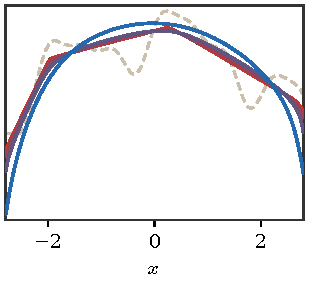
\includegraphics[width=.31\linewidth]{figures/sinkhorn-phi-soft-c-transforms--kl.pdf} &
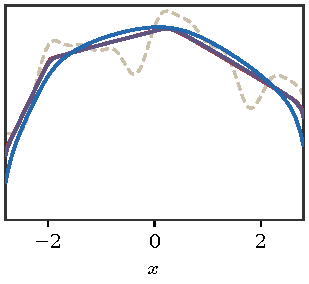
\includegraphics[width=.31\linewidth]{figures/sinkhorn-phi-soft-c-transforms--burg.pdf} &
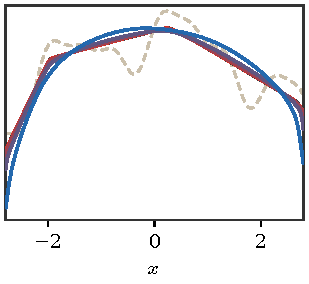
\includegraphics[width=.31\linewidth]{figures/sinkhorn-phi-soft-c-transforms--quadratic.pdf} \\[-.1em]
\small KL &
\small Burg &
\small quadratic
\end{tabular}
\caption{\emph{Generalized soft double transforms for $c(x,y)=-xy$.} Each panel starts from the same dashed non-concave potential $f$. The dark curve is the hard double $c$-transform, i.e. the concave envelope associated with the zero-temperature limit, after centering by an additive constant. Colored curves show the centered double transform $(f^{c,\epsilon,\phi})^{\bar c,\epsilon,\phi}$ from a near-zero red regularization to larger blue regularization. The numerical $\epsilon$ scale is chosen separately for each generator because KL, Burg, and quadratic density-ratio penalties have different stiffness; in each panel the red curve matches the hard concave envelope. Changing $\phi$ changes the scalar soft-normalization law and hence the way the dual ascent step smooths the envelope.}
\index{soft!c-transform}% strictindex
\index{concave envelope}% strictindex
\label{fig:sinkhorn-phi-soft-c-transforms}
\end{figure}

Figure~\ref{fig:sinkhorn-entropic-versus-quadratic-regularization} shows the corresponding change in the concentration and support of the primal coupling; its right panel is the sparse quadratic plan computed by the alternating threshold transforms above.

\begin{figure}[ht]
\centering
\setlength{\tabcolsep}{2pt}
\begin{tabular}{@{}ccc@{}}
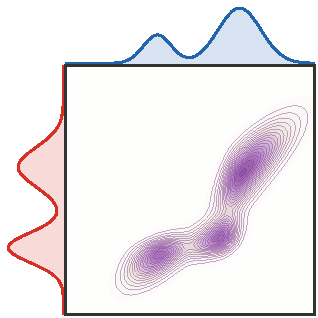
\includegraphics[width=.31\linewidth]{figures/sinkhorn-entropic-versus-quadratic-regularization--kl-plan.pdf} &
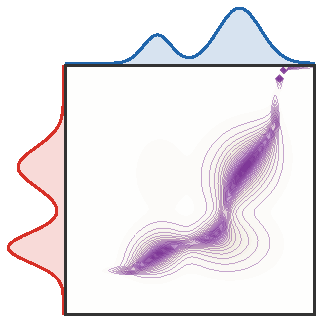
\includegraphics[width=.31\linewidth]{figures/sinkhorn-entropic-versus-quadratic-regularization--burg-plan.pdf} &
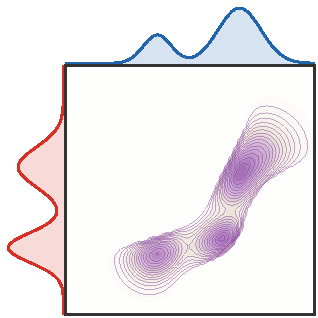
\includegraphics[width=.31\linewidth]{figures/sinkhorn-entropic-versus-quadratic-regularization--quadratic-plan.pdf} \\[-.1em]
\small $\phi(r)=r\log r-r+1$ &
\small $\phi(r)=r-\log r-1$ &
\small $\phi(r)=\frac12(r-1)^2$
\end{tabular}
\caption{\emph{Density-ratio regularizers and coupling support.} The red and blue side curves are fixed one-dimensional Gaussian-mixture marginals. Dense violet level sets display the square root of the coupling density on a common scale, using the smaller regularization strength $\epsilon=.06$. KL regularization gives the usual diffuse positive plan, the Burg barrier keeps a positive but differently tailed support, and alternate dual maximization with the quadratic soft $c$-transform produces the sparse rightmost plan through its positive-part law.}
\index{Gaussian!mixture}% strictindex
\index{density!ratio}% strictindex
\label{fig:sinkhorn-entropic-versus-quadratic-regularization}
\end{figure}

%%%%%%%%%%%%%%%%%%%%%%%%%%%%%%%%%%%%%%%%%%%%%%%%%%%%%%%%%%%%%%%%%%%%%%%%%%%

%%%%%%%%%%%%%%%%%%%%%%%%%%%%%%%%%%%%%%%%%%%%%%%%%%%%%%%%%%%%%%%%%%%%%%%%%%%
\section{Sinkhorn Divergences}
\index{Sinkhorn!divergence}% strictindex
\label{sec-sinkhorn-div}


Sinkhorn divergences remove the entropic self-bias while retaining smoothness. Under the kernel assumptions stated below, they interpolate between OT geometry and a Hilbertian energy distance, which explains their useful statistical behavior~\cite{feydy2018interpolating}.

\paragraph{Entropic bias.}
\index{entropic!bias}% strictindex

A basic defect of the raw entropic value is its self-interaction bias. Even when $c(x,x)=0$, one generally has $\MK_\c^\epsilon(\al,\al)>0$ for a non-Dirac measure. For a non-atomic $\al$, the diagonal coupling is singular with respect to $\al\otimes\al$ and has infinite relative entropy; for a discrete non-Dirac measure, it has finite but positive relative entropy. Consequently, a minimizer
\eq{
	\be_\epsilon\in\uargmin{\be}\MK_\c^\epsilon(\al,\be)
}
need not equal $\al$ for $\epsilon>0$. The following proposition identifies the high-temperature mechanism behind this bias.
\index{entropic!regularization}% strictindex

\begin{prop}[Large-temperature entropic bias]
\index{entropic!bias}% strictindex
		Let $\Xx,\Yy$ be compact and assume that $c$ is continuous. Then $\MK_\c^\epsilon(\al,\be) \rightarrow \iint c(x,y)\d\al(x)\d\be(y)$ as $\epsilon \rightarrow +\infty$.
\end{prop}
\begin{proof}
	Let $(f_\epsilon,g_\epsilon)$ be optimal dual potentials, normalized by $\int g_\epsilon\d\be=0$. The soft $c$-transform equation gives
\index{soft!c-transform}% strictindex
\index{dual!potential}% strictindex
	\[
		f_\epsilon(x)
		=
		-\epsilon\log\int
		\exp\!\left(\frac{g_\epsilon(y)-c(x,y)}{\epsilon}\right)\d\be(y).
	\]
	For bounded $c$, the oscillations of normalized entropic potentials are bounded uniformly in $\epsilon$ by the oscillation of $c$. Hence the log-sum-exp expansion is uniform:
\index{log-sum-exp}% strictindex
\index{entropic!potential}% strictindex
	\[
		f_\epsilon(x)
		=
		-\int (g_\epsilon(y)-c(x,y))\d\be(y)+O(\epsilon^{-1})
		=
		\int c(x,y)\d\be(y)+O(\epsilon^{-1}).
	\]
	At optimality the exponential penalty in the dual integrates to zero, so
	\[
		\MK_\c^\epsilon(\al,\be)
		=
		\int f_\epsilon\d\al+\int g_\epsilon\d\be
		=
		\iint c(x,y)\d\al(x)\d\be(y)+O(\epsilon^{-1}).
	\]
	This proves the limit.
\end{proof}

Thus, at large $\epsilon$, the raw entropic cost approaches the bilinear cross-energy $(\al,\be)\mapsto\iint c\,\d\al\d\be$, not a distance. The following example makes the resulting collapse mechanism explicit and then specializes it to quadratic costs.

\begin{example}[Large temperature collapse]
	Suppose that minimizers $\be_\epsilon$ are tight and that the large-temperature convergence is uniform enough to pass to their cluster points. The limiting functional is linear in the second argument:
	\[
		\be\mapsto \int V_\al(y)\d\be(y),
		\qquad
		V_\al(y)\eqdef\int c(x,y)\d\al(x).
	\]
	Thus every cluster point is supported on $\argmin V_\al$. When this set is the singleton $\{y^\star(\al)\}$,
	\[
		\be_\epsilon \rightharpoonup \delta_{y^\star(\al)},
		\qquad
		y^\star(\al)=\uargmin{y} V_\al(y).
	\]
	For the quadratic cost $c(x,y)=\norm{x-y}^2$ on $\RR^d$, assuming $\al$ has finite second moment, one has $V_\al(y)=\norm{y-\int x\d\al(x)}^2+\mathrm{const}$, so the collapse is toward the Dirac mass at the mean of $\al$.
\end{example}

\paragraph{Sinkhorn divergences.}
\index{Sinkhorn!divergence}% strictindex

The raw entropic OT value has a large-temperature attraction toward the product coupling. The standard debiasing of~\cite{feydy2018interpolating} subtracts the two self-interaction energies, in the same spirit as passing from a positive kernel value to the associated squared distance.
\index{entropic!OT}% strictindex
\index{energy!interaction}% strictindex
\index{product!coupling}% strictindex
\index{kernel!positive}% strictindex

\begin{defn}[Sinkhorn divergence]\label{def-sinkhorn-divergence}
\index{Sinkhorn!divergence}% strictindex
	Let $c$ be a symmetric cost on a common state space. For $\epsilon>0$, the debiased Sinkhorn divergence associated with the entropic OT value $\MK_\c^\epsilon$ is
	\eql{\label{eq-sinkhorn-divergence}
		\bar\MK_\c^\epsilon(\al,\be) \eqdef
		\MK_\c^\epsilon(\al,\be) - \frac{1}{2} \MK_\c^\epsilon(\al,\al) - \frac{1}{2}\MK_\c^\epsilon(\be,\be).
	}
\end{defn}
Although this formula is a debiasing by self-costs, its non-negativity is not automatic from the definition; Proposition~\ref{prop-sinkhorn-positive} proves it below by a kernel Cauchy--Schwarz argument.

\begin{rem}[Reference-measure invariance]\label{rem-sinkhorn-reference-invariance}
	The product reference in~\eqref{eq-entropic-generic} is convenient but not intrinsic to the debiased quantity. Let $\eta$ and $\zeta$ be auxiliary probability measures on the common state space such that $\al\ll\eta$, $\be\ll\zeta$ and $\KL(\al|\eta)+\KL(\be|\zeta)<+\infty$, and denote by
	\[
		\MK_{c;\eta\otimes\zeta}^\epsilon(\al,\be)
		\eqdef
		\inf_{\pi\in\Couplings(\al,\be)}
		\left\{
			\int c\,\d\pi+\epsilon\KL(\pi|\eta\otimes\zeta)
		\right\}
	\]
	the entropic value computed with this auxiliary reference. The measure-theoretic chain rule underlying Proposition~\ref{prop-kl-shift} gives, whenever the values are finite,
	\[
		\MK_{c;\eta\otimes\zeta}^\epsilon(\al,\be)
		=
		\MK_c^\epsilon(\al,\be)
		+\epsilon\KL(\al|\eta)+\epsilon\KL(\be|\zeta).
	\]
	Consequently, the marginal corrections cancel exactly:
	\begin{equation}\label{eq-sinkhorn-reference-invariance}
		\bar\MK_c^\epsilon(\al,\be)
		=
		\MK_{c;\eta\otimes\zeta}^\epsilon(\al,\be)
		-\frac12\MK_{c;\eta\otimes\eta}^\epsilon(\al,\al)
		-\frac12\MK_{c;\zeta\otimes\zeta}^\epsilon(\be,\be).
	\end{equation}
	Thus the Sinkhorn divergence is independent of the compatible product references used to compute its three terms. Mutual absolute continuity is sufficient but unnecessary; the required direction is $\al\ll\eta$ and $\be\ll\zeta$, together with finite marginal relative entropies, while reverse domination alone does not suffice. Consistency is essential: the same $\eta$ must be used in the cross-term and the $\al$ self-term, and similarly $\zeta$ must be used in the cross-term and the $\be$ self-term.
\end{rem}

Figure~\ref{fig:sinkhorn-divergence-debiasing} demonstrates the role of the two self-cost corrections by optimizing a finite point cloud against a fixed target with and without debiasing.

\begin{figure}[ht]
\centering
\setlength{\tabcolsep}{1.5pt}
\begin{tabular}{@{}cccc@{}}
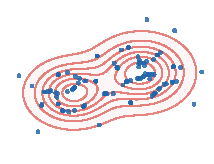
\includegraphics[width=.235\linewidth]{figures/sinkhorn-divergence-debiasing--raw-small.pdf} &
\index{Sinkhorn!divergence}% strictindex
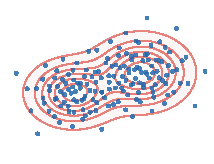
\includegraphics[width=.235\linewidth]{figures/sinkhorn-divergence-debiasing--debiased-small.pdf} &
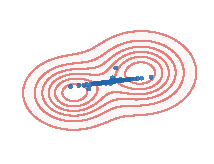
\includegraphics[width=.235\linewidth]{figures/sinkhorn-divergence-debiasing--raw-large.pdf} &
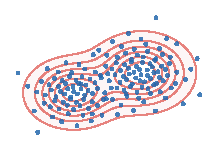
\includegraphics[width=.235\linewidth]{figures/sinkhorn-divergence-debiasing--debiased-large.pdf} \\[-.1em]
\small $\MK_\c^\epsilon$, small $\epsilon$ &
\small $\bar\MK_\c^\epsilon$, small $\epsilon$ &
\small $\MK_\c^\epsilon$, large $\epsilon$ &
\small $\bar\MK_\c^\epsilon$, large $\epsilon$
\end{tabular}
\caption{\emph{Visualization of the debiasing effect by point optimization.} The red level sets show a fixed two-Gaussian target density $\be$, while the blue atoms are an optimized empirical measure $\al_n$ initialized in the same way in all panels. For small $\epsilon$, the entropic cost $\MK_\c^\epsilon$ and the debiased Sinkhorn divergence $\bar\MK_\c^\epsilon$ both keep the two overlapping modes. For large $\epsilon$, minimizing $\MK_\c^\epsilon$ collapses the atoms toward the barycenter predicted by the large-temperature bias, whereas the self-cost subtraction in~\eqref{eq-sinkhorn-divergence} keeps a bimodal cloud.}
\index{Sinkhorn!divergence}% strictindex
\index{empirical!measure}% strictindex
\label{fig:sinkhorn-divergence-debiasing}
\end{figure}

We first record a fundamental lemma: at an optimal dual pair, the exponential regularization term integrates to zero, so the entropic cost can be read directly from the potentials. The same cancellation holds along Sinkhorn iterations after each exact block update.
\index{Sinkhorn!iteration}% strictindex

\begin{lem}[Entropic dual cost at optimum]
	Let $(f_{\al,\be},g_{\al,\be})$ be optimal dual potentials, normalized arbitrarily. Then
\index{dual!potential}% strictindex
	\eql{\label{eq-formula-cost-dual}
		\MK_\c^\epsilon(\al,\be) = \dotp{f_{\al,\be}}{\al} + \dotp{g_{\al,\be}}{\be}.
	}
\end{lem}
\begin{proof}
	We first notice that at optimality, the relation
	\eq{
		f_{\al,\be} = -\epsilon\log\int_\Yy e^{\frac{g_{\al,\be}(y)-c(x,y)}{\epsilon}} \d\be(y)
	}
	after taking the exponential, equivalently reads
	\eq{
		1 = \int_\Yy e^{\frac{f_{\al,\be}(x) + g_{\al,\be}(y)-c(x,y)}{\epsilon}} \d\be(y)
		\qarrq
			\int_{\Xx\times\Yy} \pa{ e^{\frac{f_{\al,\be} \oplus g_{\al,\be}-c}{\epsilon}} -1 } \d(\al \otimes \be) = 0.
	}
	Substituting this identity in~\eqref{eq-dual-sinkh-cont} gives the result.
\end{proof}

The next proposition records the two limiting regimes of this debiased quantity.

\begin{prop}[Asymptotics of Sinkhorn divergences]\label{prop-sinkhorn-divergence-asymptotics}
\index{Sinkhorn!divergence}% strictindex
	Let $\Xx$ be a compact metric space, let $\al,\be\in\Pp(\Xx)$, and assume that $c:\Xx\times\Xx\to\RR_+$ is continuous and symmetric, with $c(x,x)=0$.
	Then $\bar\MK_\c^\epsilon(\al,\be) \rightarrow \MK_\c(\al,\be)$ when $\epsilon\rightarrow 0$ and
	\eq{
		\bar\MK_\c^\epsilon(\al,\be) \rightarrow
		\frac{1}{2}\int -c \d(\al-\be) \otimes \d(\al-\be)
		\qwhenq
		\epsilon \rightarrow +\infty.
	}
\end{prop}
\begin{proof}
	The discrete convergence result above gives the finite-dimensional analogue; we now pass to continuous measures.
	\textbf{Case $\epsilon \rightarrow 0$.}
	The first limit is the $\Gamma$-convergence of entropic OT to the Kantorovich problem~\cite{leonard2012schrodinger,2017-carlier-SIMA}. Non-negativity of the relative entropy and continuity of $c$ give the liminf inequality. For the matching limsup, one approximates an optimal coupling by finite-entropy couplings and chooses the approximation scale so that its entropy multiplied by $\epsilon$ tends to zero. Since $c(x,x)=0$, the two self-costs in the debiased expression converge to zero, while the cross term converges to $\MK_\c(\al,\be)$.
\index{lower semicontinuity}% strictindex

	\textbf{Case $\epsilon \rightarrow +\infty$.} We denote by $(f_\epsilon,g_\epsilon)$ optimal dual potentials. After normalizing them and using boundedness of $c$, their oscillations stay uniformly bounded, so the following expansion is uniform. The optimality condition on $f_\epsilon$ (equivalently the Sinkhorn fixed point on $f_\epsilon$) reads
\index{dual!potential}% strictindex
		\begin{align*}
			f_\epsilon &= -\epsilon \log \int \exp\pa{ \frac{g_\epsilon(y) - c(\cdot,y)}{\epsilon} } \d \be(y)
			=	-\epsilon \log \int \pa{ 1 + \frac{g_\epsilon(y) - c(\cdot,y)}{\epsilon} + o(1/\epsilon) } \d \be(y) \\
			&=	-\epsilon \log\pa{1+\frac{1}{\epsilon}\int (g_\epsilon(y)-c(\cdot,y))\d\be(y)+o(1/\epsilon)}
			= - \int g_\epsilon \d\be + \int c(\cdot,y) \d \be(y) + o(1).
		\end{align*}
	Plugging this relation in the dual expression~\eqref{eq-formula-cost-dual}
	\eq{
		\MK_\c^\epsilon(\al,\be) = \int f_\epsilon \d\al + \int g_\epsilon \d \be =
		\iint c(x,y) \d\al(x)\d\be(y) + o(1).
	}
	Applying this expansion to $(\al,\be)$, $(\al,\al)$ and $(\be,\be)$ gives
	\[
		\bar\MK_\c^\epsilon(\al,\be)
		\to
		\int c\,\d\al\otimes\d\be
		-\frac12\int c\,\d\al\otimes\d\al
		-\frac12\int c\,\d\be\otimes\d\be
		=
		-\frac12\int c\,\d(\al-\be)\otimes\d(\al-\be).
	\]
\end{proof}

\begin{rem}[Large-temperature Hilbertian limit]
\index{Hilbertian!limit}% strictindex
		If $c$ is conditionally negative definite, equivalently if $-c$ is conditionally positive definite, the large-temperature limit in Proposition~\ref{prop-sinkhorn-divergence-asymptotics} is a squared Hilbertian seminorm on zero-mass signed measures. A typical example is $c(x,y)=\norm{x-y}^p$ for $0<p<2$, which yields the energy distance. This kernel norm is the dual of a homogeneous Sobolev norm.
\index{conditionally negative definite kernel}% strictindex
\index{homogeneous Sobolev norm}% strictindex
\index{Sobolev norm}% strictindex
\index{kernel!norm}% strictindex
\index{kernel!positive definite}% strictindex
\index{large-temperature limit}% strictindex
\index{Sinkhorn!divergence}% strictindex
\index{energy distance}% strictindex
\end{rem}

We now show that this debiased Sinkhorn divergence is positive.

\begin{prop}[Positivity of Sinkhorn divergences]\label{prop-sinkhorn-positive}
	Assume that the entropic dual admits optimal potentials and that the symmetric kernel $k_\epsilon(x,y)=e^{-c(x,y)/\epsilon}$ is positive semidefinite in the sense of Definition~\ref{def-positive-kernels}. Then $\bar\MK_\c^\epsilon(\al,\be)\geq0$.
	If, in addition, the common state space is compact, $c$ is continuous, and $k_\epsilon$ is universal, then $\bar\MK_\c^\epsilon(\al,\be)=0$ if and only if $\al=\be$, and $\bar\MK_\c^\epsilon(\al_n,\al)\to0$ is equivalent to $\al_n\rightharpoonup\al$.
\end{prop}

\begin{proof}
	In the following, we denote by $(f_{\al,\be},g_{\al,\be})$ optimal dual potentials for the
\index{dual!potential}% strictindex
	dual Schr\"odinger problem between $\al$ and $\be$.
\index{Schrodinger@Schr\"odinger!problem}% strictindex
	We denote by $f_{\al,\al}=g_{\al,\al}$ (one can assume they are equal by symmetry) the solution for the problem between $\al$ and itself.
	%
	Using the suboptimal function $(f_{\al,\al},g_{\be,\be})$ in the dual maximization problem, and using relation~\eqref{eq-formula-cost-dual} for the simplified expression of the dual cost, one obtains
	\eq{
		\MK_\c^\epsilon(\al,\be) \geq \dotp{f_{\al,\al}}{\al} + \dotp{g_{\be,\be}}{\be}
			 - \epsilon \dotp{ e^{\frac{f_{\al,\al} \oplus g_{\be,\be}-c}{\epsilon}} -1 }{\al \otimes \be}
	}
	Moreover $\dotp{f_{\al,\al}}{\al} = \frac{1}{2}\MK_\c^\epsilon(\al,\al)$, and similarly for $\be$, so the previous inequality equivalently reads
	\eq{
		\frac{1}{\epsilon} \bar \MK_\c^\epsilon(\al,\be)
			\geq 	1 - \dotp{ e^{\frac{f_{\al,\al} \oplus g_{\be,\be}-c}{\epsilon}} }{\al \otimes \be}
			= 1 - \dotp{\tilde\al}{\tilde\be}_{k_\epsilon}
	}
		where $\tilde\al=e^{f_{\al,\al}/\epsilon} \al$, $\tilde\be=e^{f_{\be,\be}/\epsilon} \be$
		and we introduced the positive-semidefinite kernel pairing
		$\dotp{\tilde\al}{\tilde\be}_{k_\epsilon} \eqdef \int k_\epsilon(x,y) \d\tilde\al(x) \d\tilde\be(y)$.
	The self Sinkhorn fixed point equation, once exponentiated, reads pointwise
\index{self Sinkhorn}% strictindex
	\[
			e^{f_{\al,\al}(x)/\epsilon}\int k_\epsilon(x,y)\d\tilde\al(y)=1
		\qquad \text{for }\al\text{-a.e. }x,
	\]
	and hence
	\eq{
		\norm{\tilde \al}_{k_\epsilon}^2
		= \dotp{\tilde\al}{\tilde\al}_{k_\epsilon}
		= \int e^{f_{\al,\al}(x)/\epsilon}
		\left(\int k_\epsilon(x,y)\d\tilde\al(y)\right)\d\al(x) = 1
	}
		and similarly $\norm{\tilde \be}_{k_\epsilon}^2=1$. Therefore, by Cauchy--Schwarz, one has
		$1 - \dotp{\tilde\al}{\tilde\be}_{k_\epsilon} \geq 0$.

	Suppose now that $k_\epsilon$ is universal and $\bar\MK_\c^\epsilon(\al,\be)=0$. Equality in the preceding bounds and in Cauchy--Schwarz implies that $\tilde\al$ and $\tilde\be$ have the same kernel mean embedding; universality gives $\tilde\al=\tilde\be\eqdef\tilde\mu$. The self-consistency equations then give $\d\al=(k_\epsilon\tilde\mu)\d\tilde\mu=\d\be$, where $(k_\epsilon\tilde\mu)(x)=\int k_\epsilon(x,y)\d\tilde\mu(y)$. Thus $\al=\be$, while the converse is immediate. Continuity of the entropic value and compactness of $\Pp(\Xx)$ yield the equivalence with weak convergence~\cite{feydy2018interpolating}.
\end{proof}
Positive semidefiniteness alone therefore guarantees only non-negativity and may leave a nontrivial null space.
\index{strict!positivity}% strictindex
\index{kernel!universal}% strictindex
\index{convergence!in law}% strictindex

%%%%%%%%%%%%%%%%%%%%%%%%%%%%%%%%%%%%%%%%%%%%%%%%%%%%%%%%%%%%%%%%%%%%%%%%%%%

\section{Complex \texorpdfstring{$\epsilon$}{epsilon}}
\label{sec-complex-epsilon}
\index{complex!epsilon}% strictindex
\index{Sinkhorn!holomorphic continuation}% strictindex
\index{holomorphic continuation}% strictindex

The Sinkhorn temperature is usually a positive real number: positivity makes the Gibbs kernel positive, gives the entropy a convex meaning, and underlies the Hilbert-metric and monotone convergence arguments of Chapter~\ref{sec-sinkhorn-advanced}. Once the equations are written as exponential fixed-point equations, however, $\epsilon$ can also be regarded locally as a complex variable. This does not produce a positive coupling or a contraction theorem; it produces a holomorphic branch of the same scaling equations near any positive real temperature.
\index{Gibbs!kernel}% strictindex
\index{matrix!scaling}% strictindex

\paragraph{Measure fixed point.}
\index{Sinkhorn!fixed point}% strictindex
\index{complex!measure}% strictindex

Let $\al\in\Pp(\Xx)$ and $\be\in\Pp(\Yy)$. For $\epsilon\in\CC\setminus\{0\}$, the continuous soft-transform equations~\eqref{eq-soft-c-cont-f}--\eqref{eq-soft-c-cont-g}, equivalently their multiplicative scaling form, remain valid verbatim for complex-valued scalings whenever the defining integrals exist and the divisions are well defined. For real $\epsilon>0$ these are the usual Sinkhorn equations. For complex $\epsilon$ they are only local analytic identities: they assert neither positivity of $\pi_\epsilon$ nor convergence of the alternating iteration.
\index{complex!Sinkhorn iteration}% strictindex

\paragraph{Discrete histograms.}
\index{histogram}% strictindex
\index{matrix!scaling}% strictindex

For discrete histograms, evaluate the Gibbs kernel entrywise at $(x_i,y_j)$. The scaling factorization~\eqref{eq-scaling-form} and Sinkhorn updates~\eqref{eq-sinkhorn} are then used verbatim over $\CC$, with the same marginal constraints and multiplicative gauge, whenever $\epsilon\neq0$ and all divisions are defined. This complexified iteration is again a local parametrization of the scaling equations, not a globally convergent algorithm.
\index{complex!Gibbs kernel}% strictindex
\index{complex!matrix scaling}% strictindex

The following finite-dimensional result is the scaling-variable counterpart of the analytic-dependence theorem of Carlier, Pegon and Tamanini~\cite[Theorem~2.1 and Remark~2.2]{CarlierPegonTamanini2023EntropicRates}. For compactly supported marginals and a continuous cost, their proof shows that normalized Schr\"odinger potentials, and hence the entropic cost, depend analytically on every real $\epsilon>0$; their Remark~2.2 explicitly records the resulting local extension to complex temperatures. We state the discrete version directly in $(\uD,\vD)$ and also allow the marginals and cost matrix to vary.

\begin{thm}[Local holomorphic continuation of Sinkhorn scalings]\label{thm-carlier-complex-sinkhorn}
\index{Sinkhorn!holomorphic continuation}% strictindex
\index{holomorphic implicit function theorem}% strictindex
	Fix positive histograms $\a^0\in\simplex_n$, $\b^0\in\simplex_m$, a finite real cost matrix $\C^0$, and a real temperature $\epsilon_0>0$. Choose positive scalings $(\uD^0,\vD^0)$ of the corresponding Sinkhorn coupling. Then there are complex neighborhoods of $(\epsilon_0,\a^0,\b^0,\C^0)$, inside the affine constraint $\sum_i \a_i=\sum_j \b_j$, and a unique holomorphic map
	\[
		(\epsilon,\a,\b,\C)\mapsto(\uD_\epsilon,\vD_\epsilon)\in\CC^n\times\CC^m
	\]
	satisfying the linear gauge $\sum_i\a_i^0u_{\epsilon,i}=\sum_i\a_i^0u_i^0$, such that
	$\P_\epsilon=\diag(\uD_\epsilon)\K_\epsilon(\C)\diag(\vD_\epsilon)$ has marginals $(\a,\b)$. In particular, the gauge-fixed scalings and $\P_\epsilon$ are holomorphic in all four arguments near the base point.
\end{thm}

\begin{proof}
	Apply the holomorphic implicit-function theorem to the $n$ row residuals, the first $m-1$ column residuals, and the gauge residual $G(\uD)=\sum_i\a_i^0(u_i-u_i^0)$. There are $n+m$ equations for the $n+m$ scaling coordinates. It remains to prove that their derivative with respect to $(\uD,\vD)$ is invertible at the base point.

	Let $(\delta\uD,\delta\vD)$ belong to its kernel and write
	\[
		r_i\eqdef\frac{\delta u_i}{u_i^0},
		\qquad
		s_j\eqdef\frac{\delta v_j}{v_j^0}.
	\]
	Since $\P^0=\diag(\uD^0)\K_{\epsilon_0}(\C^0)\diag(\vD^0)$, the induced perturbation is $\delta\P_{i,j}=\P^0_{i,j}(r_i+s_j)$.
	The linearized row sums vanish. The first $m-1$ linearized column sums vanish by definition of the residuals, and the last one vanishes because the total row sum equals the total column sum. Therefore
	\[
		0
		=
		\sum_i \overline{r_i}\sum_j\delta \P_{i,j}
		+
		\sum_j \overline{s_j}\sum_i\delta \P_{i,j}
		=
		\sum_{i,j}\P^0_{i,j}\abs{r_i+s_j}^2 .
	\]
	Strict positivity of $\P^0$ gives $r_i=\theta$ and $s_j=-\theta$ for some $\theta\in\CC$. The linearized gauge is $0=\sum_i\a_i^0\delta u_i=\theta\sum_i\a_i^0u_i^0$; its last factor is positive, hence $\theta=0$. The derivative is injective and therefore invertible. The implicit-function theorem now gives the asserted holomorphic scalings, and their matrix product gives the holomorphic coupling.
\end{proof}

After shrinking the neighborhoods if necessary, the scaling coordinates remain nonzero. Choosing their local logarithms defines the holomorphic log-scalings $\fD_\epsilon\eqdef\epsilon\log\uD_\epsilon$ and $\gD_\epsilon\eqdef\epsilon\log\vD_\epsilon$. These derived quantities are convenient for visualization but are not needed in the theorem.

\begin{rem}[Local, not global, complex scaling]
\index{complex!Sinkhorn scaling}% strictindex
	The theorem is local around a positive real point. It does not rule out complex singularities, changes of logarithm branch, or zeros in the denominators of the complexified updates~\eqref{eq-sinkhorn} farther away. Along a compact interval $[\epsilon_{\min},\epsilon_{\max}]\subset(0,+\infty)$, uniqueness lets the local branches agree on overlaps and therefore cover some neighborhood of that interval. This still gives no global single-valued continuation on $\CC\setminus\{0\}$.
\end{rem}

Figure~\ref{fig:sinkhorn-complex-epsilon-continuation} visualizes the continuation at the level of the coupling, without choosing logarithm branches. For a fixed real part $\epsilon_0$, it displays $\abs{\P_{\epsilon_0+i\eta}}$ at four increasing imaginary parts. The complex matrix $\P_{\epsilon_0+i\eta}$ always has marginals $(\a,\b)$, but taking its entrywise modulus destroys these linear identities. The red and blue side profiles therefore show the prescribed marginals, while the violet profiles show the row and column sums of $\abs{\P_{\epsilon_0+i\eta}}$ and reveal the cancellations hidden by the modulus.

\begin{figure}[ht]
\centering
\setlength{\tabcolsep}{2pt}
\begin{tabular}{@{}cccc@{}}
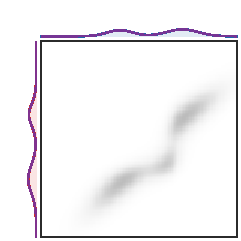
\includegraphics[width=.242\linewidth]{figures/sinkhorn-complex-epsilon-continuation--eta-0p00.pdf} &
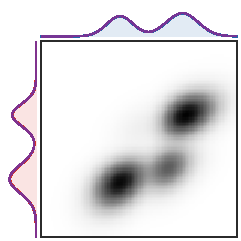
\includegraphics[width=.242\linewidth]{figures/sinkhorn-complex-epsilon-continuation--eta-0p20.pdf} &
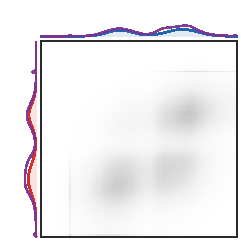
\includegraphics[width=.242\linewidth]{figures/sinkhorn-complex-epsilon-continuation--eta-0p40.pdf} &
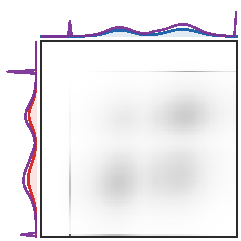
\includegraphics[width=.242\linewidth]{figures/sinkhorn-complex-epsilon-continuation--eta-0p60.pdf} \\[-.1em]
\small $\eta=0$ & \small $\eta=0.20$ & \small $\eta=0.40$ & \small $\eta=0.60$
\end{tabular}
\caption{\emph{The magnitude of a complex Sinkhorn coupling exposes the oscillations created by an imaginary temperature.} Two Gaussian-mixture histograms and $\epsilon_0=0.12$ are fixed, while $\epsilon=\epsilon_0+i\eta$ is continued through four nonnegative values of $\eta$. Every panel uses the same intensity scale. The attached red and blue profiles are the prescribed marginals $(\a,\b)$ of the complex coupling; the violet profiles are the marginals of its entrywise modulus and separate from them as cancellation increases.}
\index{complex!Sinkhorn coupling}% strictindex
\index{Sinkhorn!holomorphic continuation}% strictindex
\label{fig:sinkhorn-complex-epsilon-continuation}
\end{figure}

\begin{example}[Centered one-dimensional Gaussians]
\index{Gaussian!complex Sinkhorn}% strictindex
\index{quadratic!scaling}% strictindex
	Let $\al=\Gaussian(0,\sigma_\al^2)$ and $\be=\Gaussian(0,\sigma_\be^2)$ on $\RR$, with $\sigma_\al,\sigma_\be>0$, and take $c(x,y)=(x-y)^2$. Proposition~\ref{prop-gaussian-sinkhorn-closed-form} shows that, for real $\epsilon>0$, the Sinkhorn coupling is Gaussian. Its analytic continuation is obtained by using the same formula: for $\Re(\epsilon)>0$, set
	\[
		k_\epsilon
		\eqdef
		\frac{\sqrt{\epsilon^2+16\sigma_\al^2\sigma_\be^2}-\epsilon}{4},
	\]
	where the square root is the holomorphic branch on the right half-plane that is positive for $\epsilon>0$. The continued coupling $\pi_\epsilon$ is a centered complex Gaussian, with covariance parameter
	\[
		\begin{pmatrix}
		\sigma_\al^2 & k_\epsilon\\
		k_\epsilon & \sigma_\be^2
		\end{pmatrix}.
	\]
	Thus no new Gaussian computation is required: one simply analytically continues the real-temperature expression. This formula is guaranteed to define the finite complex Gaussian coupling throughout $\Re(\epsilon)>0$. It can be continued farther along paths on which the Gaussian integral converges and which avoid $\epsilon=0$ and the square-root branch points $\epsilon=\pm4i\sigma_\al\sigma_\be$.
\end{example}
